\documentclass[review]{elsarticle}
%\documentclass{elsarticle}

\usepackage{lineno,hyperref}
\usepackage{subcaption}
\usepackage{amsmath}
\usepackage{float}
\modulolinenumbers[5]

\DeclareMathOperator{\sgn}{sgn}

\journal{CMAME}

%%%%%%%%%%%%%%%%%%%%%%%
%% Elsevier bibliography styles
%%%%%%%%%%%%%%%%%%%%%%%
%% To change the style, put a % in front of the second line of the current style and
%% remove the % from the second line of the style you would like to use.
%%%%%%%%%%%%%%%%%%%%%%%

%% Numbered
%\bibliographystyle{model1-num-names}

%% Numbered without titles
%\bibliographystyle{model1a-num-names}

%% Harvard
%\bibliographystyle{model2-names.bst}\biboptions{authoryear}

%% Vancouver numbered
%\usepackage{numcompress}\bibliographystyle{model3-num-names}

%% Vancouver name/year
%\usepackage{numcompress}\bibliographystyle{model4-names}\biboptions{authoryear}

%% APA style
%\bibliographystyle{model5-names}\biboptions{authoryear}

%% AMA style
%\usepackage{numcompress}\bibliographystyle{model6-num-names}

%% `Elsevier LaTeX' style
\bibliographystyle{elsarticle-num}
%%%%%%%%%%%%%%%%%%%%%%%

\begin{document}

\begin{frontmatter}

\title{Heuristic and Eulerian Interface Capturing Approaches for Shallow Water Type Flow and Application to Granular Flows}


%% Group authors per affiliation:
\author[maeaddress]{Hossein Aghakhani}
\author[sandiaaddress]{Keith Dalbey}
\author[maeaddress]{David Salac}
\author[maeaddress]{Abani K. Patra\corref{correspondingauthor}}

\cortext[correspondingauthor]{Corresponding author}
\ead{abani@buffalo.edu}

\address[maeaddress]{Department of Mechanical and Aerospace Engineering, University at Buffalo, Buffalo, New York, United States}
\address[sandiaaddress]{Sandia National Laboratories, Albuquerque, New Mexico, United States}

\begin{abstract}
Determining the wet-dry boundary and avoiding the related spurious thin-layer problem when 
solving the depth-averaged shallow-water (SW) equations (or similar granular flow models) remains an outstanding challenge, though it  has 
been the focus of much research effort. In this paper, we introduce the use of level set and phase field based methods to address this issue and related problems. We also propose new heuristic 
methods to address this problem. We implemented all of these methods in TITAN2D, which is a parallel adaptive mesh refinement toolkit designed for numerical simulation of granular flows. 
Results of the methods for flow over a simple inclined plane and Colima volcano are used to illustrate the methods. For the inclined plane,
 we compared the results with experimental data and for Colima volcano they are compared to field data. Our approaches successfully captured the interface of the flow and solved the accuracy and stability problems related to the thin layer problem in 
SW numerical solution. The comparison of results shows that although all of the methods can be used to address this problem, 
each of them has its own advantages/disadvantages and methods have to be chosen carefully for each problem. 
\end{abstract}

\begin{keyword}

Shallow water flow \sep Thin layer \sep Wetting/Drying \sep Phase field \sep Level Set

\end{keyword}

\end{frontmatter}

\linenumbers

\section{Introduction} 
\label{introduction}
% Basic introduction about the Shallow water
%%{\bf NEED MORE CITATIONS}
Shallow water (SW) flows include a wide range of fluid flows in which the fluid depth is much 
smaller (${\cal O}(10^{-1})$) than the characteristic length of the fluid body. The shallowness of flow allows us to approximate the variation of state variables in the direction perpendicular to the basal surface by an integrated average \cite{SavageHutter}, which thus
reduces a three dimension flow problem into a two-dimensional one.
This approximation holds for many geophysical flows and the same 
conservation equations with  minor variations can be used to study different physical situations.
Eglit and Sveshnikova \cite{eglit1980mms} modified the depth-averaged Saint Venant equations for water flows to simulate granular snow avalanches and almost a decade later 
Savage and Hutter \cite{SavageHutter} popularized these in the modeling of many geophysical mass flows related to landslides, avalanches and debris flows. 
% introducing WD problem
Since this type of flow has free moving boundaries, identifying the location of the flow interface is a critical challenge for successful numerical methods. 
Furthermore, the governing equations are valid only in the wet areas so we need a strategy to discriminate between wet and dry areas in the numerical simulation. 
In the SW context, this is usually called the {\it wetting and drying (WD)} problem. %or {\it thin-Layer} problem 
In our previous work\cite{Patra2005}, we showed the advantages of modifying the speed of waves near the vacuum region based on Toro's approach \cite{ToroBook2001}   to mitigate stability concerns. However, this still leads to the formation of a non-physical thin layer in the numerical solution (see figure \ref{thinlayerproblem} for an illustration).
This unphysical thin layer could extend large distances from the realistic main 
body of the flow, which can cause inaccurate construction of the boundary, loss of conservation or severe 
numerical instabilities in the numerical solution. 
Besides the numerical issues, determining probable flow extents through numerical simulation is critical for application of SW equations to 
geophysical flow. For example, in preparing a hazard map 
for a volcano or a flood, it is crucial to know the location of the front of the flow to answer basic questions such as --  Does the flow reach a specific location? What is the distance of high 
risk locations from civil infrastructure? 
The answer of all the above questions is not possible without good information about the interface of the flow along its flow path.
\begin{figure}[t]
  \begin{minipage}[b]{.45\textwidth}
    \centering
    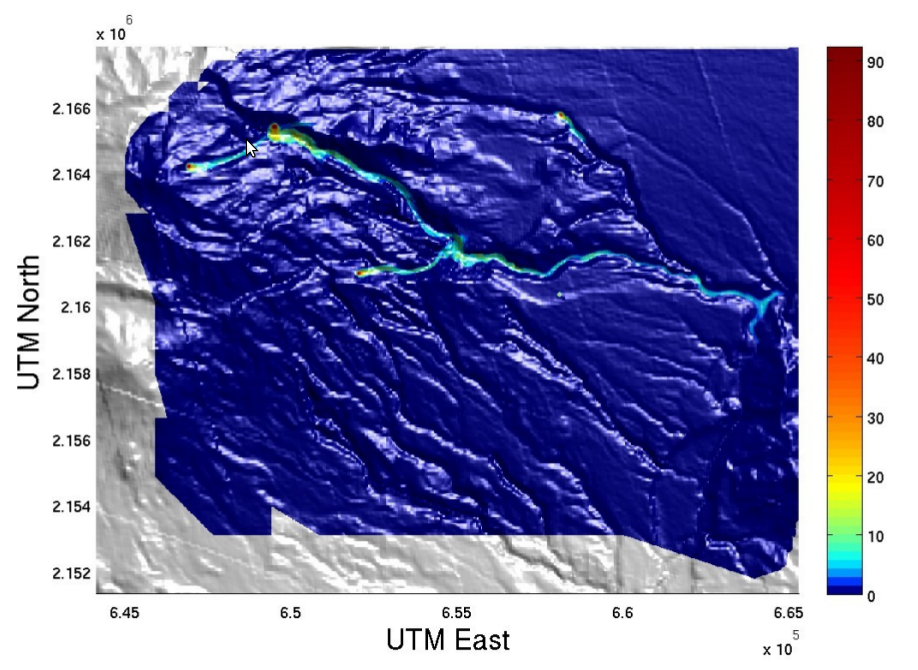
\includegraphics[width=1\textwidth]{IMAGES/rupps1.png}  
    \subcaption{ Result without any control. A thin layer of flow covers most of the domain. }
     \label{thinlayerproblem_a}
  \end{minipage}
\hspace{0.5cm}
%   \hfill
  \begin{minipage}[b]{.45\textwidth}
    \centering
    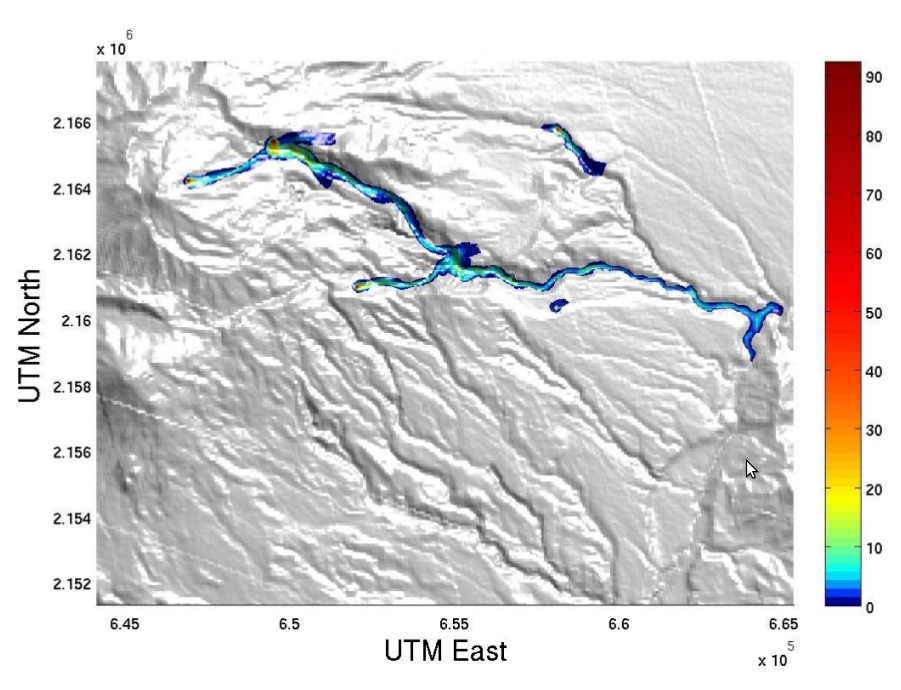
\includegraphics[width=1\textwidth]{IMAGES/rupps2.png}
    \subcaption{Only flow with depth greater than 0.5 m is displayed.}
    \label{thinlayerproblem_b}
   \end{minipage}
  \caption{Thin layer problem in maximum over time flow depth simulation of the 1955 debris flow at Atenquique, Mexico \cite{Dalbey2009}.}
  \label{thinlayerproblem}
\end{figure}
A demonstration of possible issues in shown in Figure \ref{thinlayerproblem}.
This figure displays the numerical simulation of a block of ash flow in Atenquique,  a village near the Colima volcano in Mexico, using a SW like model based on a granular flow assumption \cite{Patra2005}. The left figure shows the numerical solution of flow height without using any control for the thin layer problem 
and the right figure shows the same result  
using a naive control -- plotting the regions with flow height $h>0.5m$ (a threshold deemed too high for hazard analysis). As can be seen in the figure \ref{thinlayerproblem_a}, if no control on the numerical solution is used a thin layer of the flow covers a huge part of the domain which causes instability and inaccuracy in the obtained results.
To summarize, the following major difficulties arise in numerical solutions of SW flows related to the WD or thin layer problem:
\begin{enumerate}
        \item {\it Ambiguous and subjective computation of flow spreads.}
        \item \label{problemwicking}
             {\it Unphysical fast estimate of the flow speed.} The state variables in the  SW equations are momentum, $\{hV_x,hV_y\}$ (product of flow height and velocity). To find flow 
             velocities, $\{V_x,V_y\}$, used during the solution process the
             momentum (often a small number) must be divided by flow depth, $h$ (also small near the flow boundary),
              which can causes a large numerical error  and results in overly large flow velocities.
        \item \label{problemtoothin}
              {\it Unphysical thin layer (orders of magnitude thinner than a grain of sand).} This results from unphysical speeds and the numerical wicking away of material.
        \item \label{problemunstable}
             {\it Loss of numerical stability.} Wave-speeds can become infinite at the flow boundary which means that flow equations lose their hyperbolicity  
              at the vacuum state interface.
\end{enumerate}\label{thinprob}

In addition to scaling issues, correctly identifying 
 interface regions will allow us to construct models for  other interesting physics (e.g. entrainment) that happens at the interface.

\subsection{Background and Review}
A review of the literature shows numerous attempts have been made to overcome these problems \cite{Medeiros2013,Balzano1998,Aureli2008,Bunya2009,Casulli2009,
Kesserwani2011,DAlpaos2007,Castro2005}.
Here we briefly review the problem and recent approaches and refer the interested reader to the references for more information.
Generally, all of the approaches can be 
categorized into two basic groups which we name heuristic methods and interface tracking/capturing methods.
The basic idea of heuristic methods  \cite{Aureli2008,Bunya2009,Castro2005,Kesserwani2011} is to reconstruct the flow interface using a
simple heuristic or simple algebraic relations. In this approach, the reconstruction may take into account the physics of the problem, but this is not required. 
For example, to mitigate the thin layer problem a threshold could be defined to control the thin layer, the entire domain could be filled with a shallow level of fluid (i.e. no interface),
the flow could be reconstructed using a threshold, or the flux could be adjusted to avoid ``thin" flows. It is possible to use any combination of these heuristic fixes.
%Most of attempts that are made to address the thin layer problem are categorized under this sort of method.
In interface tracking/capturing approaches
an auxiliary set of equations is coupled to the original problem and used to follow the flow interface over time. 
%Unlike heuristic method in interface tracking/capturing methods one can find the interface of a moving boundary flow in a rigorous way. 
The particular choice of the auxiliary equations leads to either interface tracking (Lagrangian) or interface capturing (Eulerian) methods.
In Lagrangian methods, the front is replaced with a set of  points   which explicitly define the location of the interface.
During each time step these points move due to the numerically computed velocity field.
Marker And Cell (MAC) \cite{Harlow1965}, Simplified Marker And Cell (SMAC) \cite{Cheng1995} and the Surface Marker \citep{Wrobel1991} methods are some examples of Lagrangian interface tracking techniques.
The accuracy of the method is highly dependent on the number of particles that form the boundary.
High computational cost, a tendency to form numerical instabilities and the inability to track complex topological changes are the significant drawbacks of Lagrangian techniques
%For more information about this group of methods please see
 \cite{Glimm1995,Unverdi1992,Osher1988,Anderson1998,hirt1981vfv}.

In the current paper, we focus  on interface capturing or Eulerian methods. In these methods, the interface is implicitly  specified by an additional scalar field  defined in the entire 
computational domain. This additional field is coupled to the other governing equations and evolves due to the underlying fluid flow field.
The level set, phase field and Volume of Fluid (VOF) methods are  popular instances of implicit/Eulerian methods.
%%%%%%%%%%%%%%%%%%%%%%%%%%%%%% VOF   %%%%%%%%%%%%%%%%%%%%%%%%%%%%%%%%%%%%%
Hirt and Nichols \cite{hirt1981vfv} were the first to propose a VOF method. 
In this method, the scalar variable is the fraction/volume of a particular fluid in each cell.
To construct the interface based on this method, an interface  reconstruction technique is performed at each time step. 
Youngs \cite{youngs1982tdm} achieved a significant improvement 
in the VOF by adding a piecewise linear interface   (PLIC) representation of the fluid boundary. 
Youngs' method has been shown to be robust and efficient, but it is only a first order scheme. 
More advanced VOF methods are also available in Gerlach \cite{gerlach2006cvf} and Gopala and van Wachem\cite{gopala2008vfm}, but these methods require more complicated logic to 
reconstruct the interface.
%%%%%%%%%%%%%%%%%%%%%%%%%% Phase field method %%%%%%%%%%%%%%%%%%%%%%%%%%%
%The last method that we will overview here is phase field method. 
The phase field method is an Eulerian interface capturing scheme where the interface is implicitly related to an order parameter which shows the phase variation on the domain \cite{Anderson1998}. 
In this method, the interface is a well-defined diffusive region between phases. 
The mass conserving Cahn-Hilliard and non-conservative Allen-Cahn formulations are two principal formulations of this method \cite{CahnHilliard1958i,CahnHilliard1958ii,Yang2006}. %The difference between these two forms is that the first one is mass conservative while the second is not.
 Mathematically, the conservative form requires a numerically challenging fourth order derivative while the other one has only second order derivatives. 
%This difference in the highest order of derivative will make the later form much easier to implement.
To date, no published work has used the phase field method to capture an interface in the shallow water equations.
%%%%%%%%%%%%%%%%%%%%%%%%%% Level Set method %%%%%%%%%%%%%%%%%%%%%%%%%%%
The Level Set method introduced by Osher and Sethian  \cite{Osher1988} is another Eulerian interface capturing technique.  In this method, the scalar variable is typically 
a signed distance function which indicates the distance of a grid point to the interface. 
Quecedo and Pastor \cite{quecedo2002rtg} is the only instance we have found of a level set based approach to mitigate the wetting-drying problem in the context of their 
 Taylor-Galerkin approach to solve the SW equations. They presented two 
different options for handling the wetting-drying areas -- a ``simple yet efficient'' method which is  heuristic method in our classification and a level set based approach. 
Although they claimed that they used the level set as the second approach, no results using the method were included in the article and
 concluded  that the level set is expensive and unnecessary for their problem.
%============= Introduction of next parts of paper =====================
\subsection{Contributions and Summary of  Methodologies Used}
In this paper, we describe an approach to the thin layer issue (problems 1-4) discussed in section \ref{introduction}, in two parts. 
The first part is to identify the interface of the 
flow and the next is to make suitable modifications to meshes, state variables and fluxes based on the results of the first part.
To identify the interface we study three different methods. The first one is a new multifaceted heuristic approach that uses a very small dimensionless threshold, which we call it {\rm\verb1GEOFLOW_TINY1}, to 
distinguish between wet and dry areas. The other methods of interface capturing that we implement are the phase field and level set approaches.
To the best of our knowledge, the two latter methods are for the first time being applied to geophysical flow. 

As there are different types of level set and phase field methods available in the 
literature, we initially use the standard level set method and the Allen-Cahn description of the phase field, and modify them as necessary for our problem. 
The details of implementation of all three methods are carefully explained.
%After finding the interface we make suitable modifications to address the other issues. 
In the heuristic approach, after finding the wet and dry cells by using {\rm\verb1GEOFLOW_TINY1}, the cells are divided 
into three groups: wet, dry and partially wet cells. Next we adjust the fluxes for the partially wet cells and then finally update the state variables for wet cells.
In the level set and phase field approaches, refining close to cells to the identified interface enables us to control the thin layer problem. 
%Details of each approach and how we select the cells for refinement are discussed in the relevant section.
We compare the numerical results to experiments of a granular SW flow over an inclined plane ending in a horizontal surface and
 field data from the Colima volcano.
 
 The results show that all of the methods can address the thin layer problem and other 
related issues. Moreover, they indicate higher accuracy can be achieved by using the interface capturing methods though the computational cost may be higher. To decrease the computational cost, we used different techniques. For example in the phase field method, we used the Allen-Cahn formulation which is computationally less 
expensive compared to the Cahn-Hilliard formulation, but it is not mass conservative. To preserve the mass, we have included a Lagrange multiplier based approach \cite{Kim2014,Yang2006}. To decrease the computational cost further, we have used an operator splitting for time integration.
Another advantage of the interface capturing methods is that they have stronger mathematical and physical structure, and more complicated physics can be coupled with the conservation equations. The heuristic methods are simple and robust and work well when properly tuned but our experience shows that finding a good threshold in the heuristic method that is appropriate for all problems is not easy.  Finally, although we have implemented these methods for dry granular  SW flows the methods themselves are applicable for other types of SW flows.
 

The structure of the rest of this paper is as follows. In the next section the shallow-water equations for geophysical flows is described. After that the common features of the solver that we used for all of the three methods are 
introduced. In section \ref{solution}, the different methods that were employed to mitigate the wetting-drying problem are explained, and finally discussion and conclusions complete the presentation.
 
 
 
 
%Results of these tests indicate that
%the heuristic approach is less expensive than the phase field and level set methods, but the interface identified using the heuristic method moves faster than the 
%experimentally obtained interface. Additionally, our analysis shows that finding a good threshold in the heuristic method that is appropriate for all problems is not easy. 
%On other hand, the interface capturing methods have stronger mathematical and physical structure, and can be coupled with the conservation equations but are computationally more expensive and harder 
%to implement. We used several techniques to decrease the computational cost. For example, in the phase field we used the Allen-Cahn formulation which is easier to implement and computationally less 
%expensive compared to the Cahn-Hilliard formulation, but it is not mass conservative. To preserve the mass we have included a Lagrange multiplier \cite{Kim2014,Yang2006} based approach. To decrease the computational cost further
% we have used an operator splitting for time integration. 
% The   results show that all of the methods can address the thin layer problem and other 
%related issues. However, the phase field results have demonstrated better consistency with the experimental and field data. 
%Finally, although we have implemented these methods for dry granular  SW flows the methods themselves are applicable for other type of SW flows.  
%
%The structure of the rest of this paper is as follows. In the next section the shallow-water equations for geophysical flows and 
%the common features of the solver that we used for all of the three methods are 
%introduced. In section \ref{solution} the different methods that were employed to mitigate the wetting-drying problem are explained. 
%Discussion and conclusions complete the presentation.
% =============================================================================
%                METHOD
% =============================================================================
\section{Governing Equations } \label{Method}
% \subsection{SWE for geophysical flows} \label{Governingequations}
The Savage-Hutter equation for geophysical flows was first introduced in the late 1980's. 
The original model has subsequently been 
improved upon by Savage-Hutter themselves as well as others  \cite{Hutter1993,Iverson1997,Gray1999,Denlinger2001,PudasainiHutter2003,SavageIverson2003}.
In our earlier work \cite{Pitman2003,Patra2005,Patra2006}, we developed the TITAN2D depth-averaged geophysical 
flow simulator.  TITAN2D is a parallel computational tool with dynamic re-partitioning, high order, slope-limiting, upwinding, 
two-dimensional Godunov solver (without splitting), with adaptive mesh refinement and Geographic Information System 
(GIS) integration which lets it use Digital Elevation Models (DEMs) of real terrain.  
While our new multi-faceted thin-layer mitigation strategies were developed in the context of TITAN2D's capabilities, 
much of this approach should be appropriate for use in depth-averaged flow solvers with different numerical implementations. 
The depth-averaged equations that TITAN2D solves are:

\begin{equation}\label{eq:governingeq}
\hspace{-.6cm}
\frac{\partial}{\partial t}
    \begin{Bmatrix}
    h\\
    hv_x\\
    hv_y
    \end{Bmatrix}
    +\frac{\partial}{\partial x}
    \begin{Bmatrix}
    hv_x\\
    hv_x^2+\frac{k_{ap}}{2} g_z h^2\\
    hv_xv_y
    \end{Bmatrix}
        +\frac{\partial}{\partial y}
    \begin{Bmatrix}
hv_y\\
hv_xv_y\\
hv_y^2+\frac{k_{ap}}{2} g_z h^2
\end{Bmatrix}
    =
    \begin{Bmatrix}
      S_h \\
      S_x \\
      S_y
    \end{Bmatrix},
  \end{equation}
  where:
\begin{displaymath}
\begin{aligned}
S_x &= g_x h  - \frac{V_x \tan(\phi_{bed})}{\sqrt{V_x^2+V_y^2}}\left(g_z h+\frac{hV_x^2}{r_x}\right) - h k_{ap}{\rm \sgn}\left({\frac{\partial V_x}{\partial y}}\right) \frac{\partial (g_zh)}{\partial y} \sin(\phi_{int}),\\
S_y  &= g_y h  - \frac{V_y \tan(\phi_{bed})}{\sqrt{V_x^2+V_y^2}}\left(g_z h+\frac{hV_y^2}{r_y}\right) - h k_{ap}{\rm \sgn}\left({\frac{\partial V_y}{\partial x}}\right) \frac{\partial (g_zh)}{\partial x} \sin(\phi_{int}),\\
k_{ap}&=2\frac{1\pm[1-cos^2\phi_{int}(1+tan^2\phi_{bed})]^{\frac{1}{2}}}{cos^2\phi_{int}}-1,
\end{aligned}
\end{displaymath}
in $k_{ap}$, $-$ corresponds to an active state $(\frac{\partial \bar{v}_x}{\partial x}+
\frac{\partial \bar{v}_y}{\partial y}>0)$, and $+$ corresponds to a passive state $(\frac{\partial \bar{v}_x}{\partial x}+
\frac{\partial \bar{v}_y}{\partial y}<0)$.

In the above equations, the coordinate system (see Figure \ref{xzeast}) is aligned such that $x$ and $y$ are directions tangential to the surface of the 3D terrain and $z$ is normal to the surface. $h$ is the flow depth in the $z$ direction. $hV_x$ and $hV_y$ are the components of ``momentum'' in $x$ and $y$ directions, respectively, and the effect of terrain elevation changes is represented by gravitational source terms. 

\begin{figure}[!t]
        \begin{center}
                 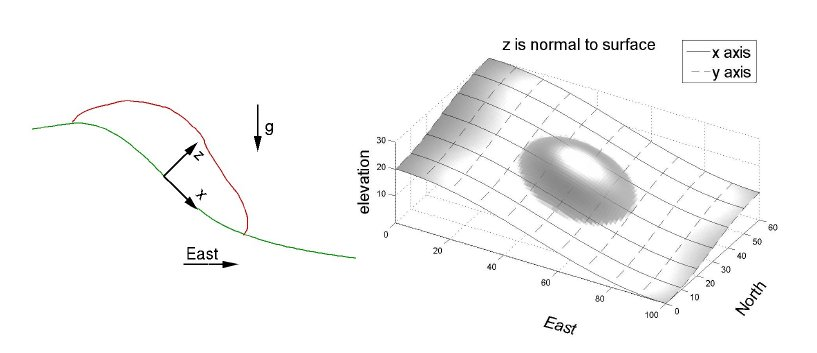
\includegraphics[width=1\textwidth]{IMAGES/1.jpg}
                \caption{In the local coordinate system the {\itshape z} direction is normal to the surface; 
                the {\itshape x} and {\itshape y} directions are tangential to the surface.}
                \label{xzeast}
        \end{center}
\end{figure}
Note that in the momentum equations $k_{ap}g_z\frac{h^2}{2}$ is the contribution of hydrostatic 
pressure to the momentum fluxes. $S_h$ is a source of mass, i.e. 
material that either effuses or erodes out of the ground. $S_x$ is 
the sum of a gravitational driving force, the friction that resists motion 
of the material relative to the bed, and the friction that resists the 
internal shearing motion of the material:

TITAN2D solves the above system of equations using a finite volume Godunov method:
\begin{equation}
   \label{integrator}
   U_i^{n+1} = U_i^n - \frac{\bigtriangleup t}{\bigtriangleup x} \{F_{i+\frac{1}{2}}^n - F_{i-\frac{1}{2}}^n \}
   - \frac{\bigtriangleup t}{\bigtriangleup y} \{G_{i+\frac{1}{2}}^n - G_{i-\frac{1}{2}}^n \}.
\end{equation}
In the above equation, G and F are the flux terms at the inter-cell boundaries which are computed by the Harten-Lax-Van Leer (HLL) \cite{Toro2009riemann} Riemann solver that is explained 
in the next section.
\section{SW Solution and Adaptive Strategy for WD Interface }
\subsection{Using Appropriate Riemann Fluxes} \label{Riemann}
Following Toro \cite{ToroBook2001}, TITAN2D uses 
the HLL Riemann average of fluxes. Let $U$ be a state variable, $F$ 
be a flux of that state variable, $s$ be a maximum wave speed, 
and $R$ and $L$ subscripts which denote ``right'' and ``left'' values 
respectively. The HLL Riemann flux is then
\begin{equation}
        F_{HLL}=\begin{cases}
                F_L & s_L\ge 0\\
                F_R & s_R\le 0\\
                \dfrac{s_RF_L-s_LF_R+s_Ls_R(U_R-U_L)}{s_R-s_L} & \textnormal{otherwise}
        \end{cases}
\end{equation}
For the Savage-Hutter system of equations the characteristic speeds are: $s_{1,3}=v\pm a$ and $s_2=v$ where $v$ is the 
velocity of fluid in the corresponding direction and $a=\sqrt{k_{ap}gh}$.
The above HLL solver is not enough for solving this system of equations.
Fraccarollo and Toro \cite{FraccarolloToro1995} note that at the 
wet-dry boundary the Riemann solution consists of a single rarefaction 
wave whose speed (when averaged over the cell length) 
is bounded above by the cell average flow speed plus 
{\bf twice} the ``speed of sound,'' $s=v+2a$, where $a=\sqrt{k_{ap}gh}$ 
for shallow water type granular flows.  They also note that ``an overestimate 
of the true wave speeds results in enhanced stability'' while an 
``underestimate of the true wave speeds could be fatal'' to stability.
They became the first to 
solve this problem by constructing an approximate Riemann solver.
\subsection{Adaptive Meshing} \label{adaptivemeshing}
In TITAN2D, each grid cell is a square or very nearly so. Rather than 
using a uniform mesh different sizes of cells are allowed, with each 
successive ``generation'' covering one fourth the area of its ``parent'' 
cell.  Note that only one generation of irregularity is allowed between 
a cell and its neighbors.
At the beginning of the simulation, \textit{i.e.} before the first update, the 
boundaries of all piles are maximally refined. An initial mesh for a 
simulation at Colima Volcano, Mexico, is displayed in Figure \ref{bufcell}. 
\begin{figure}[!h]
        \begin{center}
                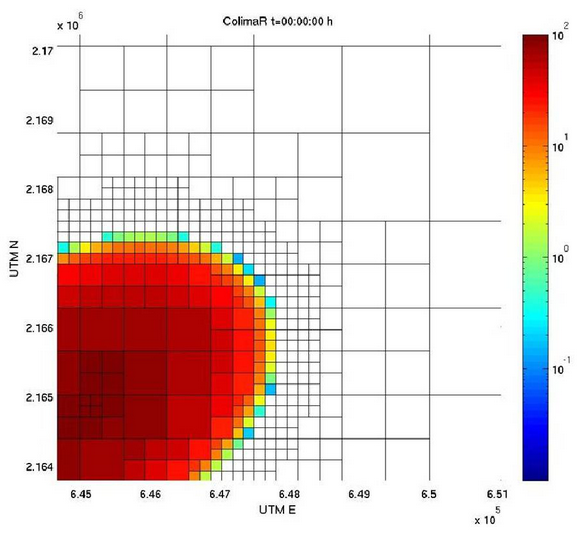
\includegraphics[scale=.3]{IMAGES/buffercells.png}
                \caption{This figure shows four layers of the maximally refined elements near the interface that we call them buffer layer. Creating buffer layers is one of the key strategies that we do to control the thin layer problem in all of the methods that we studied in this work.}
                \label{bufcell}
        \end{center}
\end{figure} 
During normal adaptivity cells are selected for refinement if they meet 
either of two requirements:
\begin{enumerate} 
        \item They have large, as compared to the average, inter-cellular fluxes.
        \item They are at or within a few cells near the interface.
\end{enumerate}
The first condition allows for the accurate capture of sharp changes in state variables. The second results in banded regions of the flow, separated into ``rings'' of maximally refined buffer cells. The number of rings are equal to or greater than the number of iterations between mesh adaptations. We usually adapt the mesh after every 5 time steps. This strategy limits artificially high transportation of material from the inside of the interface to outside of the interface and guarantees that material will only flow into maximally refined dry 
cells at the wet-dry front. However, some material that is outside of the recognized boundary may be left outside the outermost band of buffer cells. These cells are not updated until the interface passes them. The rings of buffer cells strategy decreases the numerical wicking problem and when combined with interface capturing scheme it is sufficient to decrease other thin layer problems to a level that  prevents the loss of stability.

Clearly this strategy depends on the way that we describe the interface. In the heuristic approach, we use flow below {\rm\verb1GEOFLOW_TINY1} for selecting the buffer layers. This threshold does not exactly show the interface, and our experience shows that it depends on the scale of the flow and may vary for different DEMs; therefore, we select 4 buffer layers each composed of 5 rings of refined cells at $h$ equal to 1, 5, 15 and 40 times of  the {\rm\verb1GEOFLOW_TINY1}.
In the level set and the phase field methods  we know the location of the interface at the time of computation. Thus we just make 2 buffer layers one exactly before and the other after the interface, each of them having 5 rings of refined cells. Knowing the interface location allows us to decrease the number of buffer layers from 4 to 2. This reduction
offsets some of the additional costs incurred in the additional computations for the interface capturing schemes.
  Unrefinement takes place immediately after refinement; a group of four ``sibling'' cells will be selected to merge into their mutual ``parent'' cell if the sum of their inter-cellular fluxes is very  low compared to the average flux.  Cells that have either just been refined or are otherwise in any of the current bands of buffer cells are immune 
to unrefinement.  
    
\section{Interface Capturing Strategies}\label{solution}
We have now reviewed the major difficulties and solution approaches for the WD problem in the solution of shallow water
equations.
For added motivation, the result of a simulation for Atenquique debris is displayed in figure \ref{thinlayerproblem}. 
The left picture is the obtained result from the solver and the right picture is the same result, but flow height is displayed 
only for flow height greater than 0.5 $m$. This picture shows that without correction the dominant part of the 
domain is filled with a thin layer  that  makes it difficult to identify the actual WD interface.
In this section, three methods to solve the WD problem which mitigate the numerical difficulties of SWE introduced above are detailed. 
\subsection{  Heuristic methods} \label{Heuristic}
Usually, heuristic methods use one or a combination of the following four strategies \cite{Medeiros2013}: 
\begin{enumerate}
        \item filling the entire computational domain with a thin layer of fluid;
        \item using a threshold to check whether a cell or a node is wet or dry 
         (or possibly partially wet), and then  making a decision to add or remove it 
         from the computational domain;
        \item employing some extrapolating strategy from the wet cells into their neighbor 
         cells to approximate the location of the interface. This method is usually called 
         volume/free-surface relationship (VFR) in the literature.
        \item Permitting fluid height to be negative, which means that it is below the topographical surface.
\end{enumerate}
Table \ref{table1} compares these heuristic methods.
\begin{center}\label{table1}
        \begin{tabular}{|p{.3\textwidth}|p{.3\textwidth}|p{.3\textwidth}|}
                \hline
                {\bf Strategy}                  & {\bf Mass Conservation}                                          & {\bf Physics} \\
                \hline
                {\bf Thin film}                 & Adequate, but requires solution reconstruction 
                & Produces a smooth and realistic wetting front     \\
                \hline 
                {\bf Cell removal}              & Dependent on numerical method for solving the equations          & Excellent, performs better on advancing front than receding front \\
                \hline
                {\bf VFR}                       & Conservative, with aid of some correction procedure              & Very good in wide verity of problems      \\
                \hline
                {\bf Allowable negative depth}  & Conservative, but performance depend on WD parameters            & Same as mass conservation      \\
                \hline
                % \caption{Comparison of different strategies for WD problem in SWE}
        \end{tabular}
\end{center}
Note that the heuristic method we use in this study can be categorized as a VFR method. 

\subsubsection{Selecting an appropriate threshold} \label{Threshold}
In this approach,  we use a very small threshold of a scaled flow height  to segregate the wet, partially wet and dry cells.
%The critical contribution of this scaling is to 
This identification allows other schemes 
 like those for flux adjustment and boundary reconstruction to identify where the flow %is merely ``thin'' and where it 
is non-physically thin, \textit{i.e.} where should they consider the boundary of
the flow to be. Consistency is the key requirement of whatever strategy we choose to
determine the scaling. That is, the
chosen strategy must be able to generate the same ``appropriate'' value
for depth scale at the beginning and at the end of a simulation.  
In a ``typical'' geological simulation, say of the collapse of a volcanic 
dome which would be modeled in TITAN2D as a``pile source'', the initial 
body of mass can be quite deep, but at the end of the simulation the 
material will likely be spread over a large area.  Hypothetically, if one 
were to scale by maximum flow depth at the beginning and end of the 
simulation, they would obtain vastly different values.  More importantly, 
if the only source of mass was an effusion of material out of the ground, 
the maximum initial flow depth would be zero, even if the total volume 
during the course of the simulation was the same as the previously 
mentioned ``pile source''.  
On the other hand, scaling by the cube root of the total volume of the 
flow being simulated is entirely consistent and is the flow depth 
scaling factor used by TITAN2D.  We do { not} claim that the cube root 
of volume is any more or less appropriate as a scaling factor than 
maximum initial flow depth commonly used in other shallow water contexts, for example 
storm surge simulation.
Having chosen a consistent scaling factor we were then able to define 
associated non-dimensional depths for negligibly thin and merely thin
flows.  If one were to assume that a particular geophysical mass flow 
event involved a volume of $10^8 [{\rm m}^3]$, it would then be 
reasonable to state that flow depths of less than $5 [{\rm cm}]$ were
both negligible and non-threatening.  This roughly equates to 
non-dimensional negligible flow depth, which we call 
{\rm\verb1GEOFLOW_TINY1}, with the value 
\begin{equation}
{\rm\verb1GEOFLOW_TINY1} = 0.0001.
\end{equation}
Using this value, and assuming
the volume used in a laboratory scale test was $1 [{\rm cm}^3]$, the 
resultant negligible flow depth would be $0.0001 [{\rm cm}]$.  As can 
be observed from these two examples, the chosen value of 
{\rm\verb1GEOFLOW_TINY1} is physically appropriate across a very large 
range of volumes.  Therefore, we use a theoretical contour at this depth 
as the boundary of the simulated flow.  %
%     \subsubsection{Thresholding} \label{thresholding}
In the introduction section we stated that unless steps are taken to 
prevent it, the numerical wicking (Problem \ref{problemwicking}) will
cause the flow to spread 1 cell every time-step even though the product
of flow speed and time-step size is less than the cell length.  In 
addition, the familiar continuum equations loose hyperbolicity (wave 
speeds tend to infinity) at the boundary between a continuous material 
and a vacuum.  Having implicitly defined the flow boundary,
we prevent calculation of state variables outside the flow, \textit{i.e.} in 
regions with flow depth below {\rm\verb1GEOFLOW_TINY1}.  
This reduces both non-physical flow 
spreading and computational cost. Note that state variables in cells 
with flow depth less than {\rm\verb1GEOFLOW_TINY1} are {\bf not} zeroed.  
% Once having made the the decision to implement the negligible flow 
% depth threshold, one is faced with choosing a value for the threshold.
% If the chosen threshold is overly large, it would impose a non-physical 
% limit to the flow.  Consequently, the previously stated value of 
% {\rm\verb1GEOFLOW_TINY1} was chosen with the intention of being 
% conservatively low.  However, this results in the negligible flow 
% depth threshold not being able to entirely circumvent the loss of 
% hyperbolicity (Problem \ref{problemunstableB} from Subsection 
% \ref{CausesSubSec}).  We compensate for this through appropriate Riemann 
% fluxes. Thresholding also decreases the numerical wicking (Problem 
% \ref{problemwicking}) at the flow boundary.
\subsubsection{Interface Reconstruction} \label{Interfacerecon}
As noted above, the use of a standard Eulerian grid imposes discrete 
fixed increments to the flow extent which contributes to the wicking problem
(Problem \ref{problemwicking} ) at the 
boundary.  Use of adaptive mesh refinement 
reduces this error by reducing the amount of the increment. 
The Lagrangian approach does not have this 
limitation. Tai et al. \cite{Tai2002} took advantage
of when they augmented their one-dimensional NOC scheme with 
Lagrangian front tracking.  However, implementing a hybrid 
Eulerian-Lagrangian scheme in two dimensions is significantly more 
complex. 
Therefore, %as part of our multi-faceted approach 
we implemented a very 
simple and inexpensive interface reconstruction and predictive 
Lagrangian front tracking scheme.  Knowledge of the interface allows
us to generate a representative average for an individual cell edge 
over the time-step and for values of state variables which are then used to 
compute inter-cellular fluxes into/out-of partially wet cells.  The 
interface reconstruction scheme is illustrated in figure \ref{interface}.
\begin{figure}[!h]
        \centerline{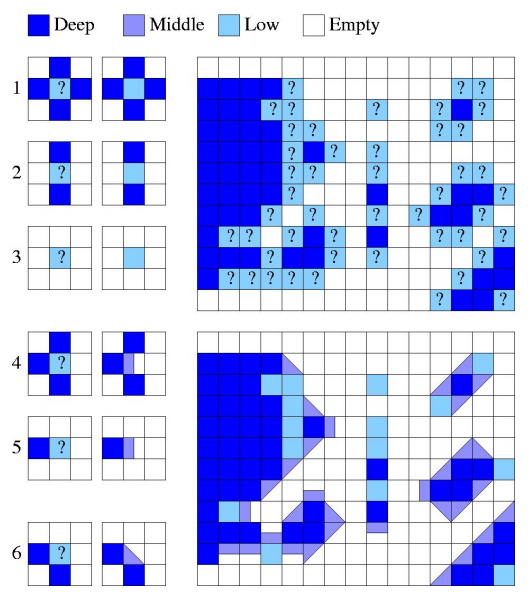
\includegraphics[scale=0.3]{IMAGES/flux.png}}
        \caption{Interface Reconstruction in TITAN2D.}
        \label{interface}
\end{figure} 
%\clearpage
Specifically, each partially wet cell is assumed to be split by a 
straight line into a completely dry and a completely wet part.  For the 
sake of simplicity, we restrict this line to one of four orientations: 
east-west, north-south, or parallel to either diagonal of the square
cell.  However, all placements/translations of the wet-dry line are 
allowed.  At the beginning of each time-step, the orientation of the 
line for the entire time-step is set based solely on which of the cell's 
neighbors have flow depth greater/less than the {\rm \verb1GEOFLOW_TINY1} 
threshold\footnote{As stated in Subsection \ref{adaptivemeshing}, the 
refinement strategy ensures that the flow front will always be maximally 
refined.  This simplifies the coding since all cells at the front can be
safely assumed to have only one neighbor on each side.}.   Orientation
of the wet-dry line, and which side of it is wet, is indicated by a single 
integer representing the geometrically determined ``most wet node.'' 
The only nine possible values for the most wet node are any of the 
cell's corners, edge midpoints or its center.  The most wet node is 
assumed to have a flow depth that is the maximum of the cell or any of 
its four neighbors.  The placement of the line is such that the volume of 
material in the cell under a plane passing through the most wet node
and the wet dry-line is the same as the unadjusted cell.  %Knowing the 
%wet-dry line's placement, the wet part only average of a conservative 
%state variables equals its whole cell average value divided by the 
%fraction of the cell's area that is wet.
Since we now know where the wet-dry line is at the beginning of the 
time step, we can compute which of the cell's edges are completely 
wet, completely dry, or partially wet, and the fraction of wetness for 
the partially wet edges.  Given the orientation and beginning of 
time-step location of the wet-dry line and the cell's state variables, 
it is also fairly straightforward to predict the line's end of 
time-step location.  This is done by convecting the wet-dry line at 
the shock speed, $s=v+a$ where the speed of sound has been adjusted 
to account for only part of the cell being wet, i.e. 
$a=\sqrt{k_{ap}gh\frac{A}{A_{wet}}}$.  Here $A$ is the whole cell's 
area and $A_{wet}$ is the portion of the cell's area that is wet.  
Since the wet-dry boundary within each partially wet cell is assumed 
to be a straight line with, during the time-step, fixed orientation, 
convecting a single point, in this case, the midpoint on the line, is 
equivalent to convecting the entire wet-dry line.  A spatial and time 
average of the wetness factor for the edge over the time-step can 
therefore be easily computed as
\begin{equation}
        W=\left(\frac{0\cdot\Delta t_{dry} +\frac{1}{2}(w_{beg}+w_{end})\Delta t_{part}+1\cdot\Delta t_{wet}}{\Delta t}\right) \left(\frac{A}{A_{wet}}\right)
        \label{wetnessfactor}
\end{equation}
where $\Delta t=\Delta t_{dry}+\Delta t_{part}+\Delta t_{wet}$ is the 
entire time-step, $\Delta t_{dry}$ is the portion of the time-step for 
which the edge is completely dry, $\Delta t_{part}$ is the portion of 
the time-step for which the edge is partially wet and partially dry, 
$\Delta t_{wet}$ is the portion of the time-step for which the edge is 
completely wet, $w_{beg}$ is the edge's fraction of wetness at the 
beginning of the time-step, and $w_{end}$ is the edge's fraction of 
wetness at the end of the time-step.
In section \ref{Interfacerecon} we explained in detail how the wet, dry and partially wet part of the cell can be computed.
 Given this information, we do not actually need to calculate the amount of time that a cell is partially wet, completely dry, 
 and completely wet. Instead, when it starts dry and ends wet, we calculate the wetness factor that we would have, 
 if we did calculate the partially wet and completely wet times. More clearly, the wet-dry line has an initial orientation and a "one-dimensional" position measured from the wettest node to the wet dry line. Moreover, we know that it is convected with constant wave speed  during the updating scheme, and we can calculate the point in time at which each node changes from wet to dry (or vice versa). Consequently, the amount of time that a cell edge is completely dry is the amount of time that both of its end points are dry and the amount of time it is completely wet is the amount of time that both  endpoints are wet.
 
\subsubsection{Adjusting Fluxes in Partially Wet Cells} \label{adjustfluxes}
The state variables used to compute the physical fluxes are the whole
cell average values multiplied by the edge wetness factor.  Note this 
results in the zeroing of this cell's physical fluxes for its sides 
that will be completely dry for the entire time-step and increasing 
them for sides that will be completely wet for the entire time-step.   
The numerical fluxes are then taken to be the HLL Riemann average of 
the ``adjusted'' physical fluxes from the cells on both sides the edge.  
The wetness factor adjustment of fluxes delays/decreases the transfer 
of material from partially wet cells to completely dry cells.  This 
delay significantly reduces the amount of non-physical flow spreading, 
and requires negligible additional computation and memory usage.  In 
terms of memory usage, this scheme only requires one additional
integer indicating the most wet node, and two additional decimal 
numbers for the cell's fraction of wet area and the location of the 
wet-dry line's midpoint (implemented as a single number ranging from 
zero to one).  The flux adjustment in partially wet cells mitigates
the numerical wicking (Problem \ref{problemwicking}) at the boundary but not within the flow (that
requires either a uniform grid or an adaptive strategy based on
fluxes and the rings of buffer cells strategy).
% 
% {\bf 1D Analysis of partially wet flux adjustment}
% 
% There are 3 cells L, M, R.  $h_R=V_R=0$, $h_L>2 h_M>0$ (the middle cell is partially wet), $V_L>0$, $V_M>0$.  The time step is set by the middle cell with a Courant number $C$. 
% 
% The wet area of the {\it partially wet} middle cell is defined as follows
% \begin{eqnarray}
% h_m A &=& \frac{1}{2} h_L A_wet  \\
% \frac{A_{wet}}{A} &=& 2\frac{h_m}{h_L}
% \end{eqnarray}
% More generally 
% \begin{equation}
% \frac{A_{wet}}{A}=\min\left(1,2\frac{h_m}{h_L}\right)
% \end{equation}
% We can then compute a wet portion average of $h$ and $hV$ for the middle cell
% \begin{eqnarray}
% \hat{h}_m&=&h_m\frac{A}{A_{wet}} \\
% \widehat{(hV)}_m &=& hV\frac{A}{A_{wet}}
% \end{eqnarray}
% The adjusted wave speeds in the middle cell are $s=V_m \pm 2\alpha\sqrt{\hat{h}_m}=V_m \pm 2 \alpha \sqrt{h_m} \sqrt{\frac{A}{A_{wet}}}$.  This makes the time step
% \begin{equation}
% \Delta t = C \frac{\Delta X_m}{V_m+2\alpha\sqrt{h}\sqrt{\frac{A}{A_{wet}}}}
% \end{equation}
% The wet-dry line can then be convected at $s=V_m+2\alpha\sqrt{h_m}\sqrt{\frac{A}{A_{wet}}}$ and the time at which the flow will reach the edge of middle and right cells.   
% \begin{eqnarray}
% \Delta t_{part} &=& \min\left(\Delta t, \frac{\Delta X_m \left(1-\frac{A_{wet}}{A}\right)} {V_m+2\alpha\sqrt{h}\sqrt{\frac{A}{A_{wet}}}}\right) \\
% \Delta t_{wet}&=&\Delta t - \Delta t_{part} 
% \end{eqnarray}
% We can then define a time averaged wetness factor, $W_{MR}$ for the middle cell for the edge shared by the middle and right cells
% \begin{eqnarray}
% W_{MR}&=&\frac{\Delta t_{wet}}{\Delta t} \frac{A}{A_{wet}}\\
% &=&\left(1-\frac{\Delta t_{part}}{\Delta t}\right)\frac{A}{A_{wet}}\\
% &=&\frac{A}{A_{wet}}-\min\left(\frac{A}{A_{wet}},\frac{\frac{\Delta X_m}{\Delta t} \left(\frac{A}{A_{wet}}-1\right)}{V_m+2\alpha\sqrt{h}\sqrt{\frac{A}{A_{wet}}}}\right)\\
% W_{MR}&=&\frac{A}{A_{wet}}-\min\left(\frac{A}{A_{wet}},\frac{1}{C}\left(\frac{A}{A_{wet}}-1\right)\right)
% \end{eqnarray}
% Then 
% \begin{eqnarray}
% F_{hMR}^*&=&\frac{\left(V_m+2\alpha\sqrt{h_m}\sqrt{\frac{A}{A_{wet}}}\right)W_{MR}h_mV_m-\left(V_m^2-4\alpha h_m\frac{A}{A_{wet}}\right)W_{MR}h_m}{4\alpha\sqrt{h_m}\sqrt{\frac{A}{A_{wet}}}}\\
% &=&\frac{W_{MR}h_m}{2}\left(V_m+2\alpha\sqrt{h}\sqrt{\frac{A}{A_{wet}}}\right)
% \end{eqnarray}
% Likewise 
% \begin{eqnarray}
% F_{hVMR}^*&=&\frac{\left(V_m+2\alpha\sqrt{h_m}\sqrt{\frac{A}{A_{wet}}}\right)\left(W_{MR}h_mV_m^2+\frac{1}{2}\alpha^2W_{MR}^2h_m^2\right)-\left(V_m^2-4\alpha h_m\frac{A}{A_{wet}}\right)W_{MR}h_mV_m}{4\alpha\sqrt{h_m}\sqrt{\frac{A}{A_{wet}}}}\\
% &=&...
% \end{eqnarray}
% 
% The middle cell's wetness factor, $W_{ML}$, for the edge shared with the left cell is
% \begin{equation}
% W_{ML}=\frac{A}{A_{wet}}
% \end{equation}
% Note that if the wet-dry line does not reach the edge shared by the middle and right cells within the time step then $W_{MR}=0$.  Assuming that this is the case then
% $h_R'=V_R'=0$ and ... 
% $h_M'$, and $V_M'$ also depend on $h_L$ and $V_L$ so their values must be known/assumed in order to compute/simplify $h_M'$ and $V_M'$
\subsection{Second: Phase Field Method} \label{phase field}
%As noted earlier, another approach that is employed 
%for capturing the interface of a SW type flow is the phase field method.
In this method, the state variables are augmented by a continuous
order parameter. This order parameter, $\varphi$, 
implicitly represents the interface in the domain. To this aim, a new transfer equation must be solved which is coupled with the other state variables. 
Papers \cite{Anderson1998,Chen2002,Boettinger2002,Kim2012} are good references about the history and evolution of the method.
Phase diffusion methods and particularly the phase field method is based upon the notion that the interface between phases is a diffusive region rather than a sharp interface. 
The value of $\phi$ is constant within a bulk phase but changes smoothly between the phases. In this work $\phi$ is 1 for the fluid phase $ \lbrace \textbf{x}: \phi(\textbf{x},t)=1 \rbrace  $, 
and it is -1 for void regions $ \lbrace \textbf{x}: \phi(\textbf{x},t)=-1 \rbrace  $, and is between -1 to 1 on the diffusion region $ \lbrace \textbf{x}: -1 < \phi(\textbf{x},t) < 1 \rbrace  $. 
We can implicitly assume the interface of the flow is where $ \lbrace \textbf{x}: \phi(\textbf{x},t)= 0 \rbrace  $.
%The strong thermodynamical and physical derivation of the method make it so powerful for capturing the complicated topological changes especially for the problems that the interface motion depends 
%on gradients of an external field normal to the interface and on the local curvature of the interface.
In this study, we have used the Allen-Cahn form of the phase field. 
\begin{equation} 
        \label{allencahn}
        \frac{\partial \varphi }{\partial t} + \overrightarrow{V}\cdot \nabla \varphi = 
        \gamma (\bigtriangleup\varphi -F'(\varphi)),
\end{equation}
where:
\begin{equation} 
        \label{fprime}
        F(\varphi)=\frac{1}{4\eta^2} (\varphi^2-1)^2 ,\text{\ so \ \ } F'(\varphi)= \frac{\delta F}{\delta \varphi} = \frac{1}{\eta^2} \varphi (\varphi^2 -1).
\end{equation}
In the above equation, $\eta$ is a constant that regulates the capillary width or diffusion width, $ \gamma $ denotes an elastic relaxation constant, and $F(\varphi)$ is 
a mixing free energy which is the well-known double-well potential function and represents the interactions of different volume fractions of individual species \cite{Bronsard1990,Larson1999}.

%{\bf THE FOLLOWING NEEDS HELP!}
This formulation is easier to solve, but is not mass conservative. To conserve the mass, we follow \cite{Kim2014,Yang2006}, and use a Lagrange multiplier $\xi(t)$ modified as $(\varphi^2-1)\xi(t)$ to enforce the depth
averaged conservation of form of the mass $ \frac{D}{Dt} \int_\Omega \varphi h \ \ dx= 0$. This results in an additional source term in  \eqref{allencahn}.
 The $(\varphi^2-1)$ modification  for the Lagrange multiplier minimizes the  change $\varphi$ on the bulk region  i.e when $\varphi=\pm1$. 
 The final form of equation \eqref{allencahn} and the constraint are:  
\begin{align} 
        \label{allencahn_mod}
        \frac{\partial \varphi }{\partial t} + \overrightarrow{V}\cdot \nabla \varphi &= 
        \gamma (\bigtriangleup\varphi -F'(\varphi)+ (\varphi^2-1)\xi(t)), \\
%\end{equation}
%and the constrain that has to be satisfied is:
%\begin{equation} 
        \label{constrain}
        \frac{D}{Dt} \int_\Omega h \varphi \ \ dx&= 0,
\end{align}
Physically \eqref{constrain} implies that the volume of pile must be constant during the simulation. A simple relationship for  $\xi(t)$ is derived as follows:
\begin{equation} 
    \begin{aligned}
        \label{eta}
        \frac{D}{Dt} \int_\Omega \varphi h \ \ dx &= h \int_\Omega \frac{D}{Dt}  \varphi  \ \ dx+\underbrace{\varphi \int_\Omega  \frac{D}{Dt} h  \ \ dx}_{=0 \text{\ \ continuity}} \\ &=h\int_\Omega \gamma (\bigtriangleup\varphi -F'(\varphi)+\varphi (\varphi^2-1)\ \xi(t)) \ \ dx=0,
            \end{aligned}
\end{equation}
The first term in above relation will be neglected by applying the Gauss' theorem for the Neuman boundary conditions($
        \frac{\partial \varphi}{\partial n}\vert_{\Gamma} = 0,
$):
\begin{equation}
        \label{lapbound}
        \int_\Omega h \gamma  \nabla. \nabla \varphi \ dx = 
        \int_\Gamma h \gamma \nabla \varphi \ ds = 0,
\end{equation}
so to always satisfy the constrain \eqref{constrain} we end up with:
\begin{equation} 
        \label{eta_cont}
\frac{1}{\eta^2} \int_\Omega  \varphi (\varphi^2 -1) \ \ dx = \xi(t) \int_\Omega (\varphi^2-1)  \ \ dx \Rightarrow \xi(t) = \frac{\int_\Omega  \varphi (\varphi^2 -1) \ \ dx}{\eta^2 \int_\Omega (\varphi^2-1)  \ \ dx }
\end{equation}
We set $\eta=n\  \delta x$, where $\delta x$ is equal to the smallest cell length of all elements and $n$ is the number of the buffer layers explained in section \ref{adaptivemeshing}.
For time integration of equation \eqref{allencahn_mod} we use operator splitting. The Euler explicit method is used for time integration of all terms except the Laplacian terms, 
which are updated implicitly. For a stable explicit time integrator, the size of the time step has to satisfy the CFL condition.

\begin{align}
\frac{\varphi^{i+.5}-\varphi^i}{\bigtriangleup t}&= \gamma (-F'(\varphi^i)+\varphi^i (1-(\varphi^i)^2)\ \xi(t^i)) \label{eq1.exp}\\
\frac{\varphi^{i+1}-\varphi^{i+.5}}{\bigtriangleup t} &= \gamma \nabla .\nabla \varphi^{i+1} \label{eq2.exp}
\end{align}
We used GMRES solver of the PETSc \cite{petsc-user-ref} library to solve equation \eqref{eq2.exp}. Since the Krylov subspace solvers just needs the result of matrix-vector multiplication, we used matrix-free method to compute the Laplacian term to decrease the memory cost of implicit solver.


\subsection{Third: Level Set Method} \label{level set}
%The last method that we use to capture the interface for a SW flow is the Level Set method.
The Level Set method is another Eulerian interface capturing method, originally introduced by Osher and Sethian  \cite{Osher1988}. There are many papers about Level Sets for  interface capturing in flow simulations \citep{Kees2011,Losasso2006,Sethian2003}, but the application of the method is not limited to these \citep{Li2011b,Lie2006}.
The basis of the method is to capture the interface by   solving a hyperbolic Hamilton-Jacobi PDE on 
the computational domain for $\varPsi (X,t)$, a signed distance function which  is zero on the interface and has an absolute value in the domain depending on the distance to the zero level.  The level set variable $\varPsi (X,t)$ implicitly represents the interface. 
 $\varPsi (X,t)$ is  positive outside  the interface and  negative inside. 
Given the initial condition $\varPsi_0 (X,t)$ the advection of the interface ($\varPsi (X,t)=0$) only depends on the normal velocity $F$:
\begin{equation}\label{levelseteq1}
        \frac{\partial \varPsi}{\partial t} + F |\nabla \varPsi| = 0,
\end{equation}
substituting $F = \overrightarrow{V} \cdot \overrightarrow{n} $ which  $\overrightarrow{n} $ is the normal vector, and is equal to
$ \frac{\nabla \varPsi}{|\nabla \varPsi|}$ leads to:
\begin{equation}\label{levelseteq2}
        \frac{\partial \varPsi}{\partial t} + \overrightarrow{V} \nabla \varPsi = 0
\end{equation}
\subsubsection{Reinitialization} \label{reinitialization}
The solution of equation \eqref{levelseteq2} might not remain a signed distance function. To keep $\varPsi$ a signed distance function, we need a procedure that is called 
reinitialization. There are several techniques for this purpose \cite{Osher1988}, but what we implemented here is a composition of the method presented in Chopp's work \cite{Chopp2001} with 
some modifications for the points close to the interface, and a PDE based reinitialization for the further places\cite{Sussman1994a}.
PDE based reinitialization is easy for parallelization, though it has been known to induce mass loss. Chopp suggests a bicubic interpolation for the points near the interface \cite{Chopp2001},
but here we use a bilinear interpolation which is not as accurate, but it is accurate enough to preserve the interface and cheaper. 
For points far from the interface we do not need a very accurate $\varPsi$, so we use a PDE based reinitialization which is easier to implement and has lower computational cost. 
In our approach, we first find $\varPsi$ for the points that are adjacent to the interface, then use these points to update the signed distance function for rest of the domain using a PDE based method.
In this way, the interface $( \varPsi=0 )$ is preserved with an affordable computational cost and effort. Moreover, since just $\varPsi$ is required for the points that are located near the interface, 
there is no need to update it for  the whole domain. So in this work we select $\varPsi_{thresh}<10\ \delta x$, where $\delta x$ is the smallest size of the elements, 
as the threshold for updating $\varPsi$ in the PDE-based reinitialization process.
The signed distance function is updated for  points  adjacent to the interface in the following steps:
\begin{enumerate}
\item First we find the adjacent points to the interface, and store them in a list that is usually called the accepted point list in the literature \cite{Chopp2001}. 
\item The next step is to determine the interpolant for the level set function, $p(X)$, that returns $\varPsi(X)$ for a point $X$.
\item The last step is to compute the distance of the accepted points based on the following conditions:
\begin{subequations}
\begin{align}
&p(X_{int})=0,\label{dist_cond1} \\ 
&\nabla p(y) \times (X_0-X_{int})=0,\label{dist_cond2}
\end{align}
\end{subequations}
where $X_{int}$ is the nearest point on the interface, and $X_0$ is the point in the accepted list that we want to compute its distance to the interface. 
The first condition \eqref{dist_cond1} requires that $X_{int}$ is on the interface, and the second condition states that the interface normal at the closest point 
must pass through $X_0$. In this part, we followed the notation of Chopp's paper \citep{Chopp2001}.
\end{enumerate}

In the first step, we just need to find those points where the sign of $\varPsi$ is different from their neighbors, and store them in a list that we call them accepted points list. 
For the second step, there are different ways to perform the interpolation. In many applications, like in this study, the initial interface has a specific geometrical shape such as a circle or ellipse, 
so we do not need to find this interpolant approximately, and its equation can be used directly as $p(X)$. 
For example, in this study the initial pile has an elliptic shape, so the initial interface follows the elliptic equation. However,
we will still have to use  approximate $p(X)$ for reinitialization as the curve evolves.

If the equation of the interface is not known, which is usually the case, approximating the interface by interpolation is necessary. Chopp suggested a bicubic approximation \cite{Chopp2001} to achieve a fully second order accurate result, but this method requires the solution of a 16 by 16 system of equations for cells containing the interface to determine the coefficients of the bicubic interpolation. 
The purpose of the interpolation based method is to ensure that the interface does not undergo spurious motion.
Therefore, the use of bilinear interpolation should be sufficient. The general form of $p$ is:
\begin{equation}\label{interpolation}
p=a_0+a_1 \ x+ a_2 \ y+ a_3 \ xy.
\end{equation} 
A general way to find $a_0$ to $a_3$ for a grid with different element sizes is to solv%e a system of 4 by 4 equations \eqref{bilin_system} 
use the value of $\varPsi$  
at cell centers of four adjoining cells (see fig. \ref{fig:bilinear_interp}).
\begin{equation}
\label{bilin_system}
\begin{bmatrix}
    1 & x_1 & y_1 & x_1 y_1 \\
    1 & x_2 & y_2 & x_2 y_2 \\
    1 & x_3 & y_3 & x_3 y_3 \\
    1 & x_4 & y_4 & x_4 y_4 \\
\end{bmatrix}
\begin{bmatrix}
    a_0 \\
    a_1 \\
    a_2 \\
    a_3
\end{bmatrix}
=
\begin{bmatrix}
    \varPsi_1  \\
   \varPsi_2  \\
    \varPsi_3  \\
     \varPsi_4  
\end{bmatrix}
\end{equation} 
In our case the elements near the interface are of uniform size, and the four cell centers can be considered as the vertices of a rectangle, so the coefficients of 
equation \eqref{interpolation} can be computed as following:
\begin{subequations}
\begin{align}
a_0&=\frac{(\varPsi_1 x_2 y_2 - \varPsi_2 x_2 y_1 - \varPsi_3 x_1 y_2 + \varPsi_4 x_1 y_1)}{(x_2-x_1)(y_2-y_1)}, \\ 
a_1&=\frac{(-\varPsi_1 y_2 + \varPsi_2 y_1 + \varPsi_3 y_2 - \varPsi_4 y_1)}{(x_2-x_1)(y_2-y_1)},\\
a_2&=\frac{(-\varPsi_1 x_2 + \varPsi_2 x_2 + \varPsi_3 x_1 - \varPsi_4 x_1 )}{(x_2-x_1)(y_2-y_1)}, \\ 
a_4&=\frac{(\varPsi_1 - \varPsi_2 - \varPsi_3 + \varPsi_4)}{(x_2-x_1)(y_2-y_1)}, \\ 
\end{align}
\end{subequations}
where $\varPsi_1=(x_1,y_1), \varPsi_2=(x_1,y_2), \varPsi_3=(x_2,y_1)$ and $\varPsi_4=(x_2,y_2)$ as can be seen in the figure \ref{fig:bilinear_interp}.
\begin{figure}[ht]
\centering
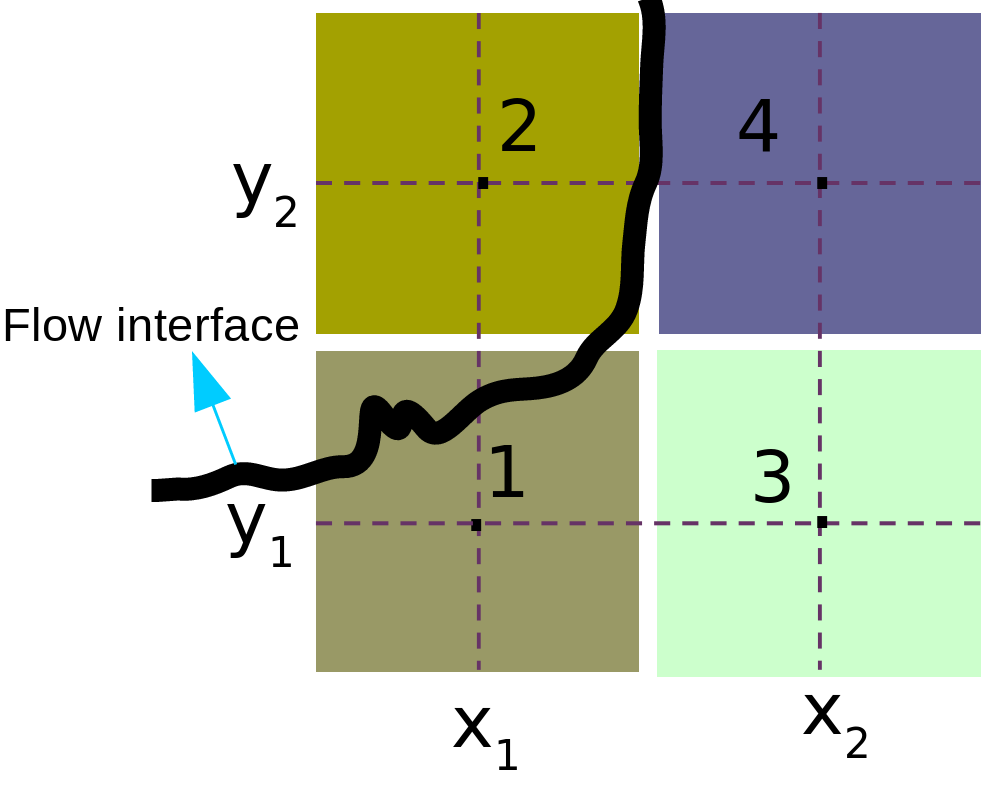
\includegraphics[scale=.15]{IMAGES/bilinear_interp.png}
\caption{Configuration of the four elements that have been selected for bilinear interpolation. In this schematic example the interface passes through two hypothetical edges of (2-4) and (1-2) edges. This is just for demonstration purpose and has no effect on the equations.}
                \label{fig:bilinear_interp}
\end{figure}
After finding the interpolation function $p$, we can compute the distance from a point to the interface using equations \eqref{dist_cond1} and \eqref{dist_cond2}. 
The solution is calculated using a variant of Newton's method as presented in \cite{Chopp2001}:
\begin{subequations}
\label{eqnewton}
\begin{align}
&\delta_1=-p(X^k)\frac{\nabla p(X^k)}{\nabla p(X^k).\nabla p(X^k)},\\
& X_{1+\frac{1}{2}}=X_k+\delta_1,\\
& \delta_2=(X^0-X^k)-\frac{(X^0-X^k).\nabla p(X^k)}{\nabla p(X^k).\nabla p(X^k)}\nabla p(X^k),\\
&X_{k+1}=X_{1+\frac{1}{2}}+\delta_2.
\end{align}
\end{subequations}
This is an iterative method that starts from $X_0$, which is the point whose distance to the interface must be determined. 
Once the nearest point on the interface is determined, the distance can be computed, and sign of $\varPsi$ is the same as it was before reinitialization.
For interpolation as shown in equation \eqref{interpolation}, we need four points. When we create the accepted list, instead of storing single points we store a pair of points that are 
neighbors whose sign of $\varPsi$ differs. Then to find two other points, it is enough to select a direction perpendicular to the direction that connects the selected pair, 
and find the neighbors of the first two points in this direction. 


Before proceeding to the PDE-based step, we would like to make some remarks about the aforementioned step. 
In parallel computation, the domain is decomposed between multiple processors, with each processor holding a port responsible for a part of the domain. 
The information on neighboring processors is stored in ``ghost"-cells, which are updated using inter-processor communication. In TITAN2D, only the neighboring ghost
cells in the $x$ and $y$ directions are provided. Thus, a cell at location $(i,j)$ does not have direct access to the information stored at location $(i+1, j+1)$. 
This causes issues in the rare instances that the interface is near the corner of a processor's domain, figure \ref{fig:surf_interp}. To avoid 
excessive inter-processor communication in these rare cases, the bilinear interpolation described before is modified to purely linear interpolation method requiring 
only three points:
\begin{equation}
\label{Surface}
p=a_0+a_1 x+a_2 y.
\end{equation} 
When choosing the three points needed for interpolation, we ensure that only the points in Cartesian directions are used.
With these three points the interpolant is given by:
\begin{figure}[ht]
\centering
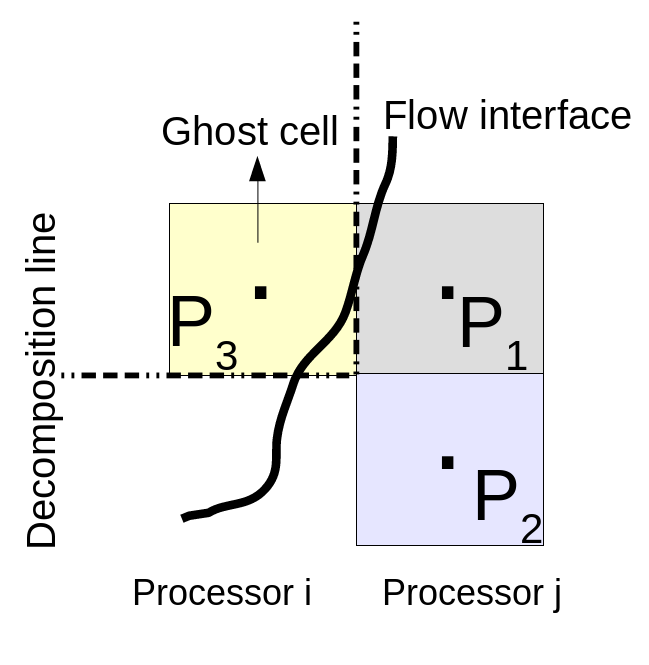
\includegraphics[scale=.25]{IMAGES/surf_interp.png}
\caption{In this figure $p_1$ and $p_2$ are updated in processor j and $p_3$ is updated in processor i, but its information is available in processor j as ghost cell. }
                \label{fig:surf_interp}
\end{figure}
\begin{align}
&p_1=
\begin{bmatrix}
    x_1 \\
    y_1 \\
    \varPsi_1
\end{bmatrix}
,\ \ 
p_2=
\begin{bmatrix}
    x_2 \\
    y_2 \\
    \varPsi_2
\end{bmatrix} 
,\ \ p_3=
\begin{bmatrix}
    x_3 \\
    y_3 \\
    \varPsi_3
\end{bmatrix}, \nonumber\\
&\overrightarrow{n}=\overrightarrow{p_2p_1}\times\overrightarrow{p_3p_1}=
\begin{bmatrix}
    n_1 \\
    n_2 \\
    n_3
\end{bmatrix}=
\begin{bmatrix}
    (y_2-y_1)(\varPsi_3-\varPsi_1)-(y_3-y_1)(\varPsi_2-\varPsi_1) \\
    (x_3-x_1)(\varPsi_2-\varPsi_1)-(x_2-x_1)(\varPsi_3-\varPsi_1) \\
    (x_2-x_1)(y_3-y_1)-(x_3-x_1)(y_2-y_1)
\end{bmatrix},\\
&a_0=\frac{n_1}{n_3}x_1+\frac{n_2}{n_3}y_1+\varPsi_1 \ \ \  \ a_1=\frac{-n_1}{n_3}, \ \ \ a_2=\frac{-n_2}{n_3}
\end{align}
Another point that we would like to make is that standardized structures, such as the set container of the C++ standard library, are useful data structures for storing the 
adjacent points near the interface. The reason for this is that this container keeps its item in a sorted way, and does not allow the storage of duplicate items. 
This simplifies the coding effort as we do not need manually to check list every time that we want to save a new element. 

After finding $\varPsi$ for the points adjacent to the interface, $\varPsi$ in other points can be updated with a PDE based reinitialization using an upwinding scheme. 
We use the following PDE for this aim:
\begin{equation}\label{initializationeq}
        \frac{\partial \varPsi}{\partial \tau} + \sgn (\varPsi_0) (|\nabla \varPsi| - 1)= 0.
\end{equation}
In equation \eqref{initializationeq}, $\tau$ is a pseudo-time and the equation should be solved until it converges reasonably. This PDE adjusts $\varPsi$ such that $|\nabla \varPsi|=1$.
We solve equation \eqref{initializationeq} by the method introduced in \cite{Adalsteinsson1999}:
\begin{equation}
        \varPsi_{ij}^{n+1}=\varPsi_{ij}^{n}-\bigtriangleup t \left(max(F,0)\bigtriangledown_{ij}^{+}+min(F,0)\bigtriangledown_{ij}^{-} \right),
\end{equation}
where 
\begin{equation}
        \begin{aligned}
                \bigtriangledown_{ij}^{+} = \big[ & \max(D^{-x}\varPsi_{ij}^{n})^2 + \min(D^{+x}\varPsi_{ij}^{n})^2
                \\& \max(D^{-y}\varPsi_{ij}^{n})^2 + \min(D^{+y}\varPsi_{ij}^{n})^2 \big]^{1/2}
        \end{aligned}
\end{equation}
\begin{equation}
        \begin{aligned}
                \bigtriangledown_{ij}^{-} = \big[ & \min(D^{-x}\varPsi_{ij}^{n})^2 + \max(D^{+x}\varPsi_{ijk}^{n})^2
                \\& \min(D^{-y}\varPsi_{ij}^{n})^2 + \max(D^{+y}\varPsi_{ij}^{n})^2 \big]^{1/2}
        \end{aligned}
\end{equation} 
In the above equations $D^+$, and $D^-$ are the backward and forward differences, respectively, in the corresponding directions.
We solve equation \eqref{initializationeq} until $\sum\limits_{ij}|\varPsi_{ij}^{n+1} -\varPsi_{ij}^{n}| < .5 (\delta x)^3$ over all points being updated.

\section{Results} \label{results}
We use two cases to illustrate the  interface capturing schemes. The first case is flow down an inclined plane while the second is past eruptions at the Colima Volcano. 
For the first case, we have access to  detailed and accurate  experimental data and careful comparisons are possible. 
The second is more characteristic of typical field observations available to calibrate and validate TITAN flows and only sparse deposit data is available.
%
%For the later one, i.e Colima Volcano, we used the field observation data of the outline and characteristic of the flow to simulate an eruption numerically and compare the results.
Since the computational cost of the methods is not the same, we have also compared these methods from a computational point of view by the required simulation time and the number of elements generated in the adaptive meshing process
during the simulation. 

\subsection{Inclined plane}
In this section, the results of the inclined plane are presented. The input parameters and initial conditions of the flow are in  table 1.
\begin{center}
        \begin{tabular}{|l|c|}
                % \caption{Initial condition}
                \hline
                Pile shape       & Cylindrical \\
                \hline
                Maximum pile height       & .061 m \\
                \hline
                Major extent of the pile  & .0525 m \\
                \hline
                Minor extent of the pile  & .0525 m \\
                \hline           
                Bed friction angle        & $32.47^o$ \\
                \hline
                Internal friction angle  & $37.3^o$ \\
                \hline
                Angle of incline          & $38.5^o$ \\
                \hline
                Physical time simulated   &  90 sec \\
                \hline
        \end{tabular}
\end{center}



\begin{figure}[!ht]
        \begin{minipage}[b]{.5\linewidth}        
                \centering
                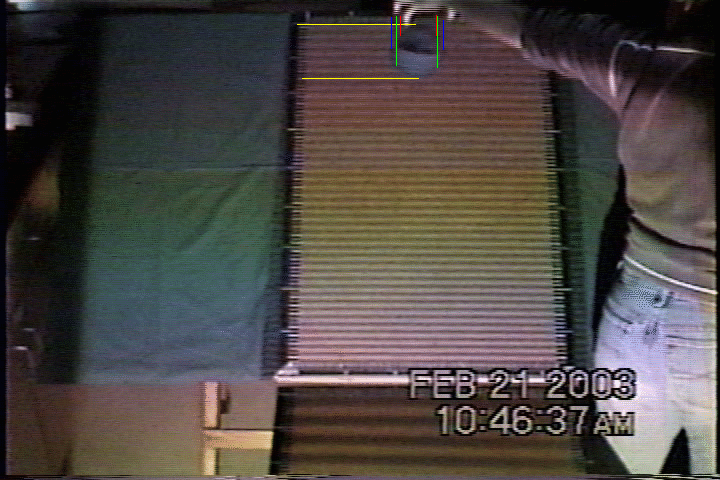
\includegraphics[width=1\textwidth]{IMAGES/expinitialconf.png}
                \subcaption{Experimental setup}
        \end{minipage}
        %   \hfill
        \begin{minipage}[b]{.5\linewidth}
                \centering
                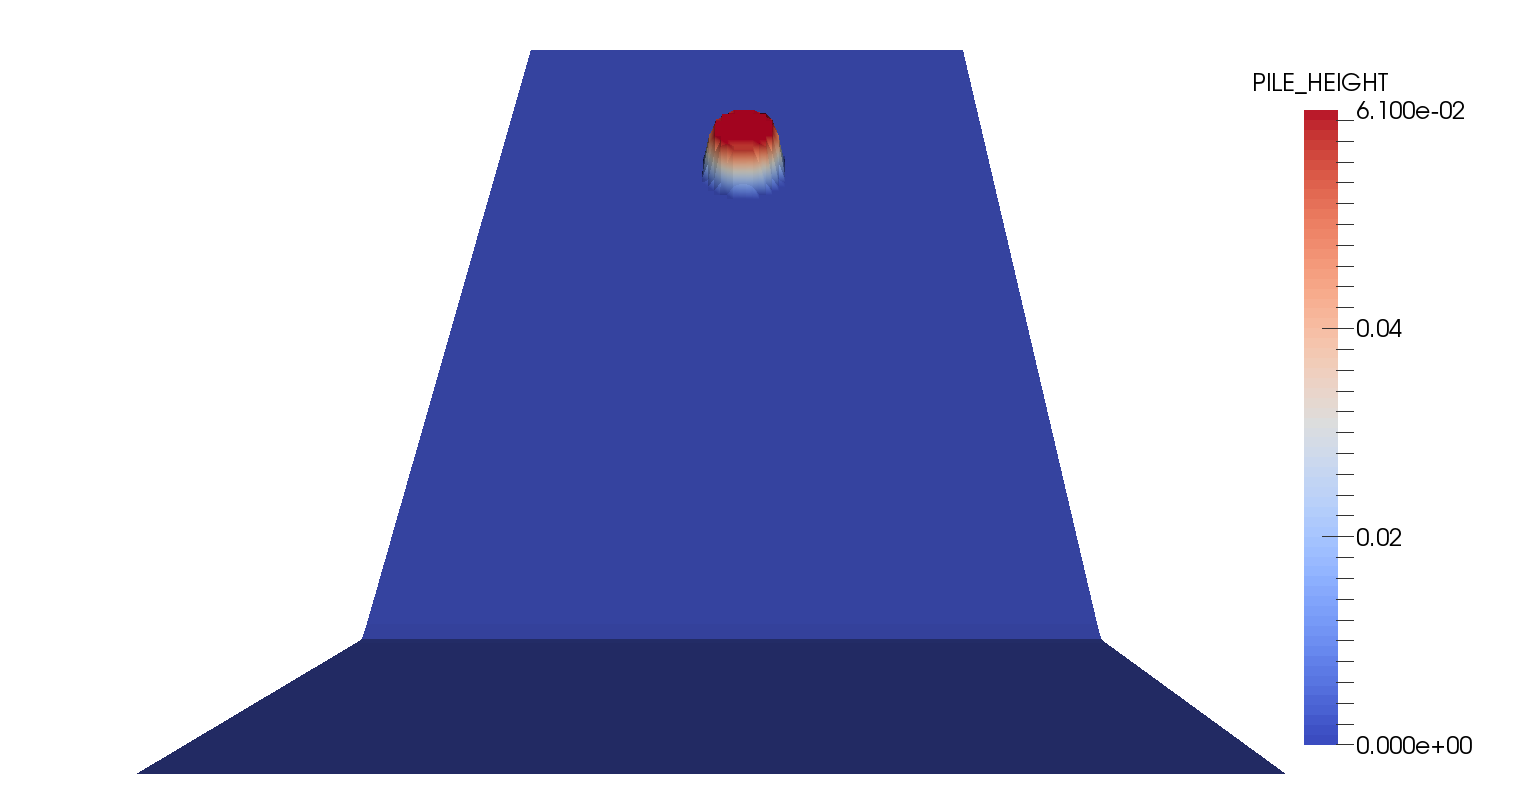
\includegraphics[width=1\textwidth]{IMAGES/initialconf.png}
                \subcaption{Numerical simulation}
        \end{minipage}
        \caption{Initial configuration of the pile on the incline.}
        \label{initialconf}
\end{figure}
%\subsubsection{Heuristic Method}
\begin{figure}[H]
        \begin{minipage}[b]{.5\textwidth}
                \centering                
                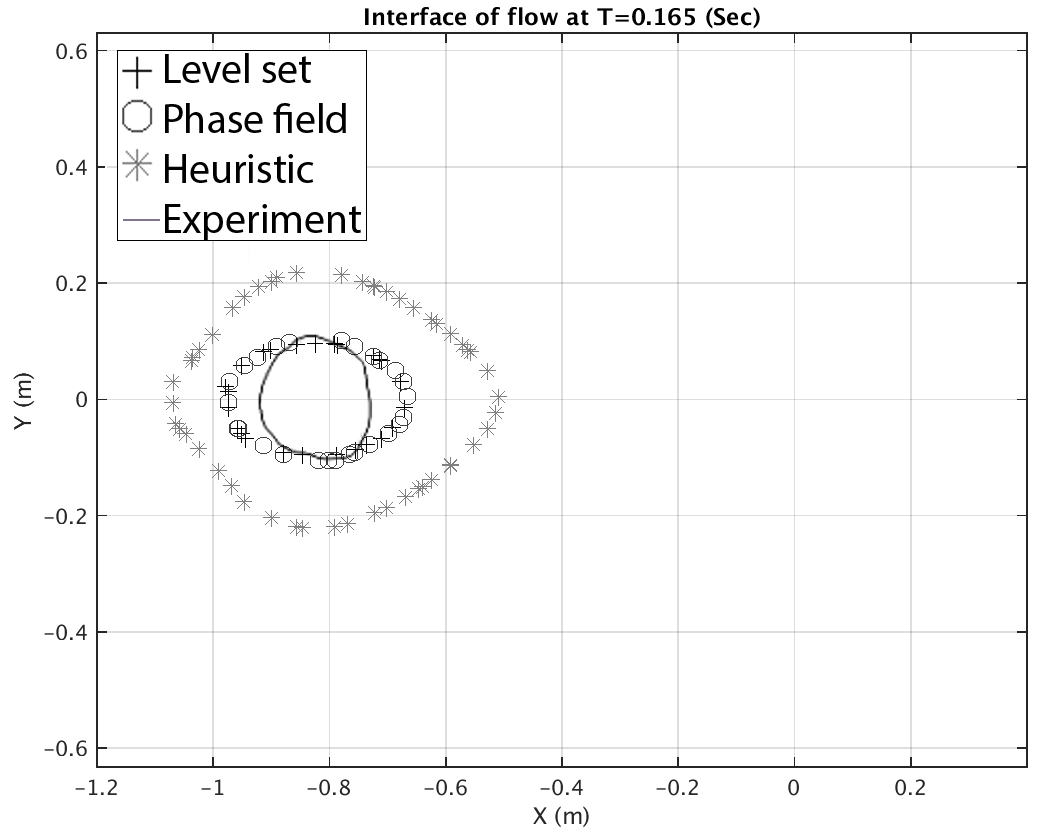
\includegraphics[width=1\textwidth]{IMAGES/interface165.png}                
                \subcaption{T=0.165 sec}              
                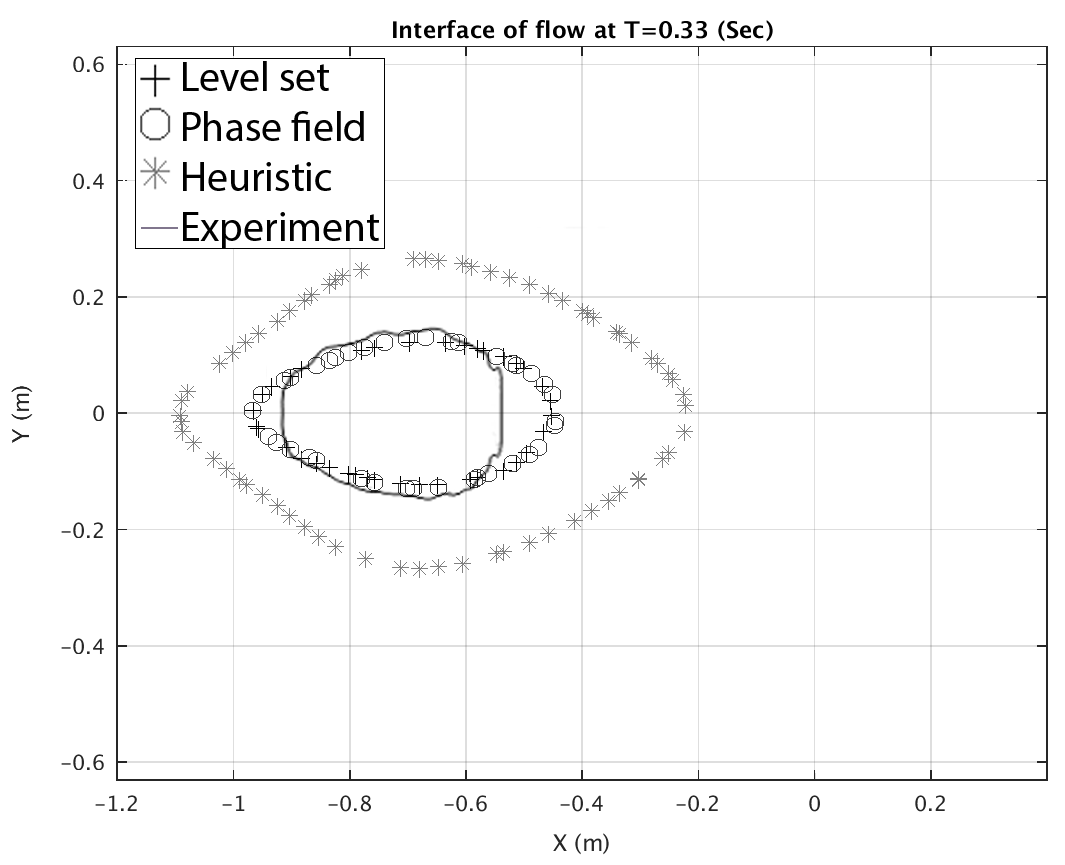
\includegraphics[width=1\textwidth]{IMAGES/interface330.png}
                \subcaption{T=0.33 sec}
              
        \end{minipage}
        %   \hfill
        \begin{minipage}[b]{.5 \textwidth}
                \centering
                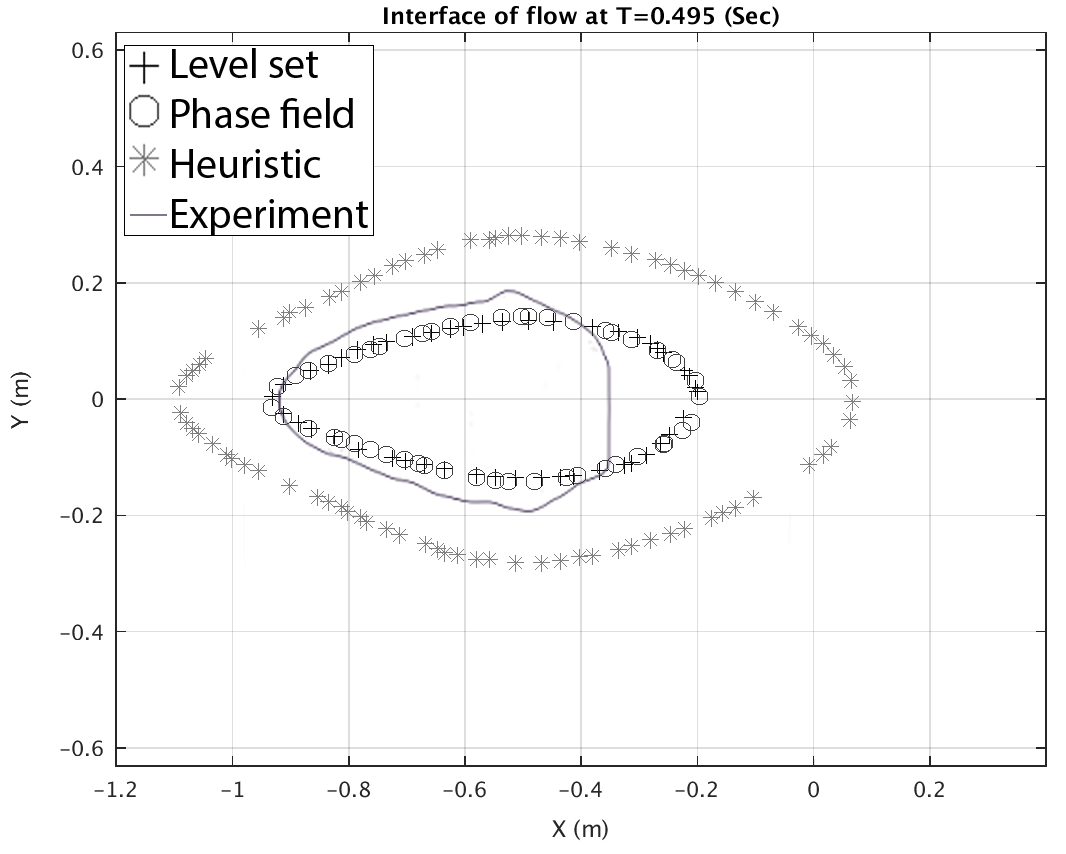
\includegraphics[width=1\textwidth]{IMAGES/interface495.png}
                \subcaption{T=0.495 sec}
                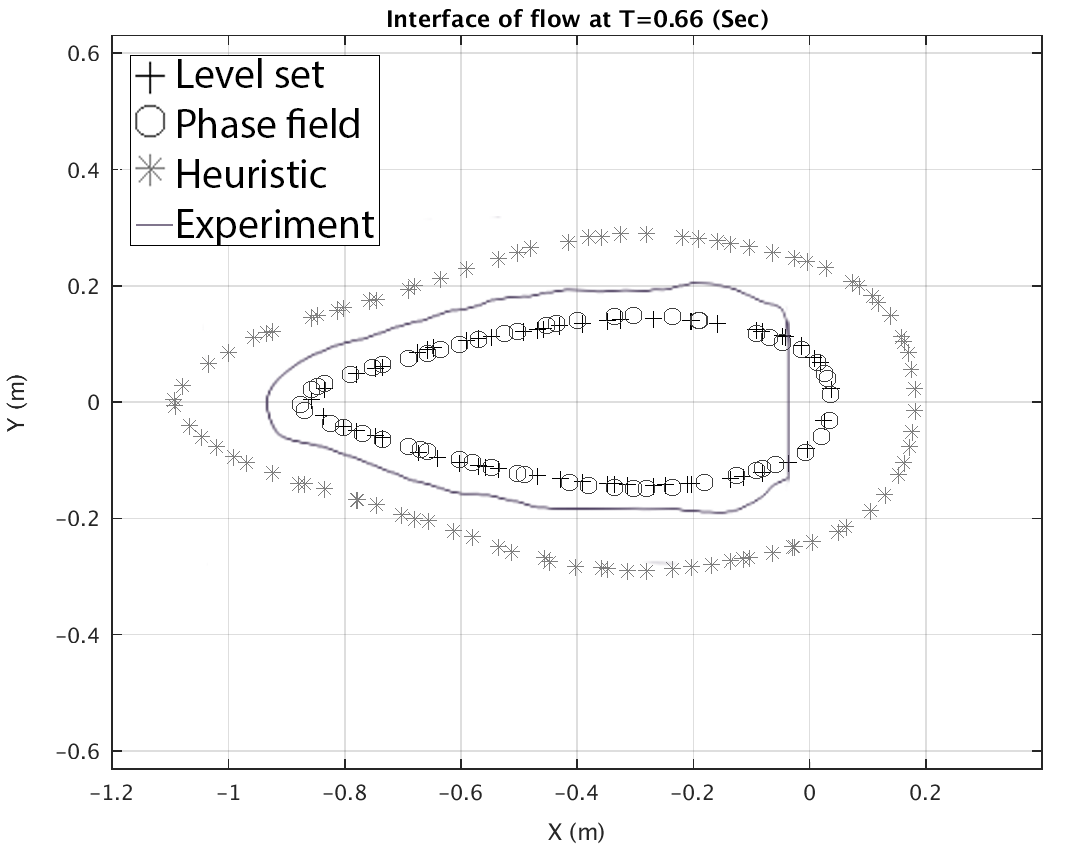
\includegraphics[width=1\textwidth]{IMAGES/interface660.png}
                \subcaption{T=0.66 sec}
        \end{minipage}
        \caption{Pile height contour and interface location at different time steps.}
        \label{Pile_height_contour}
\end{figure}
The experimental results were reported in \cite{AmyWebb2004}, and we have used them to verify   numerical results  in previous work. 
Figure \ref{initialconf} shows the initial configuration of the pile in both the experimental setup and the numerical study. As can be seen in the experimental setup, 
there are markers in the inclined plane that are used for measurements. Webb \cite{AmyWebb2004}
  used a digital camera and image processing techniques to compute the extents of the flow in 
x and y directions as well as its area and perimeter, and then compared the obtained results with the numerical simulations.% in figure \ref{compinc_inclined}.  
The raw data from observation was re-analyzed in the course of this investigation and the actual flow depth data was updated to account for a small error in the original calculations
reported in \cite{AmyWebb2004}.
We also plotted 
the interface of the flow for the three interface capturing schemes and the experimental results in figure \ref{Pile_height_contour}.
The plotted interfaces in figure \ref{Pile_height_contour} are for $\phi=0$ and $\varPsi=0$ for the Phase Field and the Level Set methods respectively 
and $h=\sqrt[3]{Vol} \times {\rm\verb1GEOFLOW_TINY1}  $ for the heuristic method where $Vol$ is the volume of flow and ${\rm\verb1GEOFLOW_TINY1} = .0001$, as was described in section \ref{Threshold}.

Figure \ref{Pile_height_contour} shows that the results of the Eulerian interface capturing schemes are very similar for the inclined plane, 
and are closer to the experiment than the heuristic method. In all four plotted time steps, the heuristic method appears to move ahead of the true  interface. 
It is possible to obtain better agreement by tuning the value of  ${\rm\verb1GEOFLOW_TINY1}  $  but in that case we will end up with a  ${\rm\verb1GEOFLOW_TINY1}$ that
 depends on the particular flow rendering the use of TITAN for anything but hindcasts problematic. 
A primary goal of  this study is to find a method that can predict the interface of a geophysical flow independent of the scale of the flow, 
and for this reason we selected two very different scales of flows (i.e flow over the inclined plane and Colima volcano), 
and the ${\rm\verb1GEOFLOW_TINY1} $ that we use here have been tested in much of our previous work, and has showed reasonable results \cite{Patra2005,Patra2006}. 

In figure \ref{x_extent} the extent of flow in X direction was plotted. This plot shows the length of flow during its travel. 
The maximum of the flow length happens when the flow reaches the horizontal plane. All of the methods are successful in predicting the time 
that flow reaches the horizontal plane, but like the interface results (figure \ref{Pile_height_contour}) the heuristic method over-predicts the length of the flow.
The Phase Field and the Level Set results are a better match with the experimental result.

The width of the flow or extent of the flow in Y direction can be seen in figure \ref{y_extent}. 
There is a much larger difference between the experiment and the Eulerian interface capturing methods results in this figure than the other results, 
and based on our previous work \cite{Patra2006}, we believe the main reason for this difference is due to the accuracy of the solver. 
In that work, we showed that with more accurate simulations using a higher order Discontinuous Galerkin method we can better capture the width of the flow.
Future work will address the combination of such higher order methods and the interface capturing schemes.

The other measure we use to compare the results is the area of the flow. 
In figure \ref{area}  one can see that the Eulerian methods capture the area of the flow fairly well,
especially before the flow hits the horizontal surface while the heuristic method over-estimates the area of the flow. 
The last result is that of the perimeter of the flow (figure \ref{Perimeter}), which shows a similar behavior 
to the other results that have been discussed earlier. 

From these results, all three methods successfully overcome the thin layer problems  (problems 1-4 section \ref{introduction}) for this simple problem, though
 the Eulerian interface capturing methods  captured the flow with significantly higher accuracy than the heuristic method.
\begin{figure}[H]
        \begin{minipage}[b]{.5\textwidth}
                \centering
                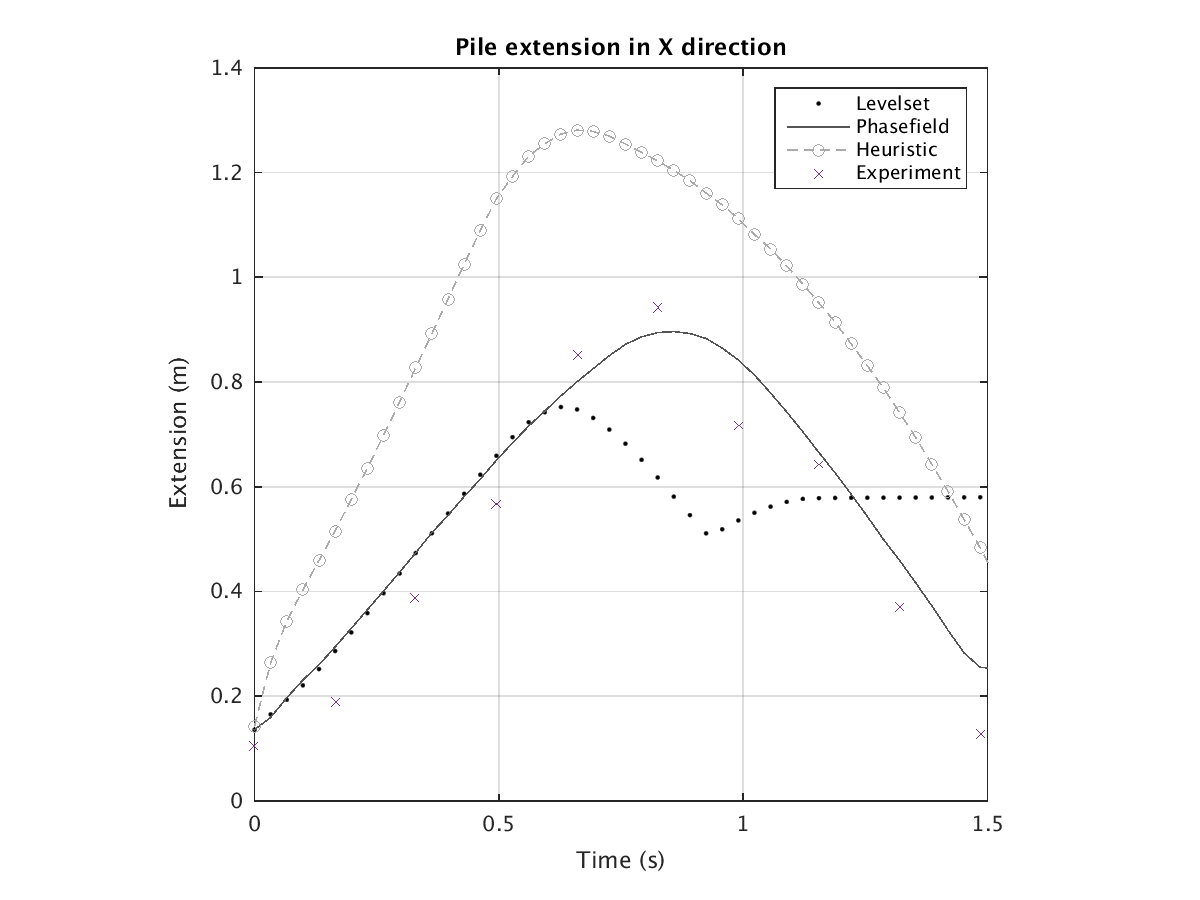
\includegraphics[width=1\textwidth]{IMAGES/xextend.png}
                \subcaption{Extension of pile in X direction.}
                  \label{x_extent}
                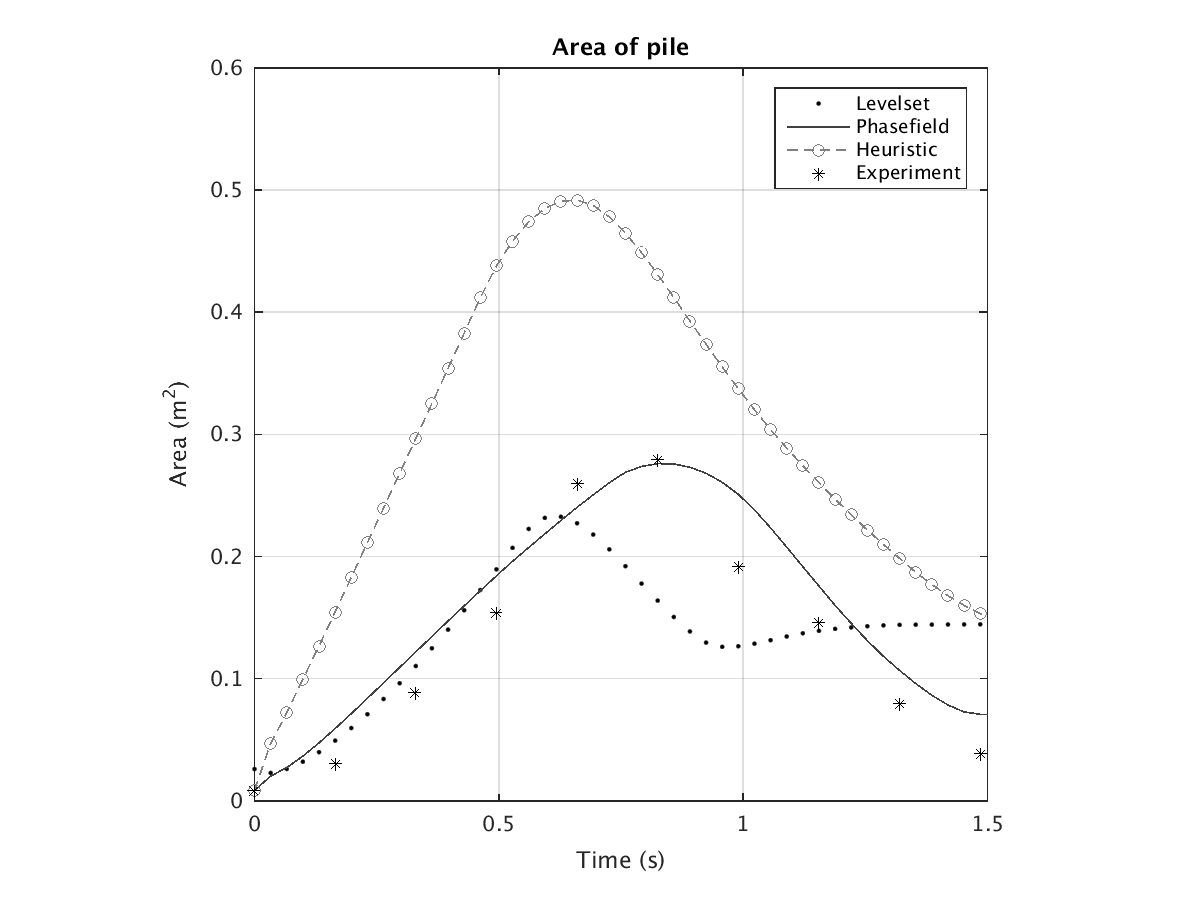
\includegraphics[width=1\textwidth]{IMAGES/area.png}
                \subcaption{Area of pile.}
                  \label{area}
        \end{minipage}
        %   \hfill
        \begin{minipage}[b]{.5\textwidth}
                \centering
                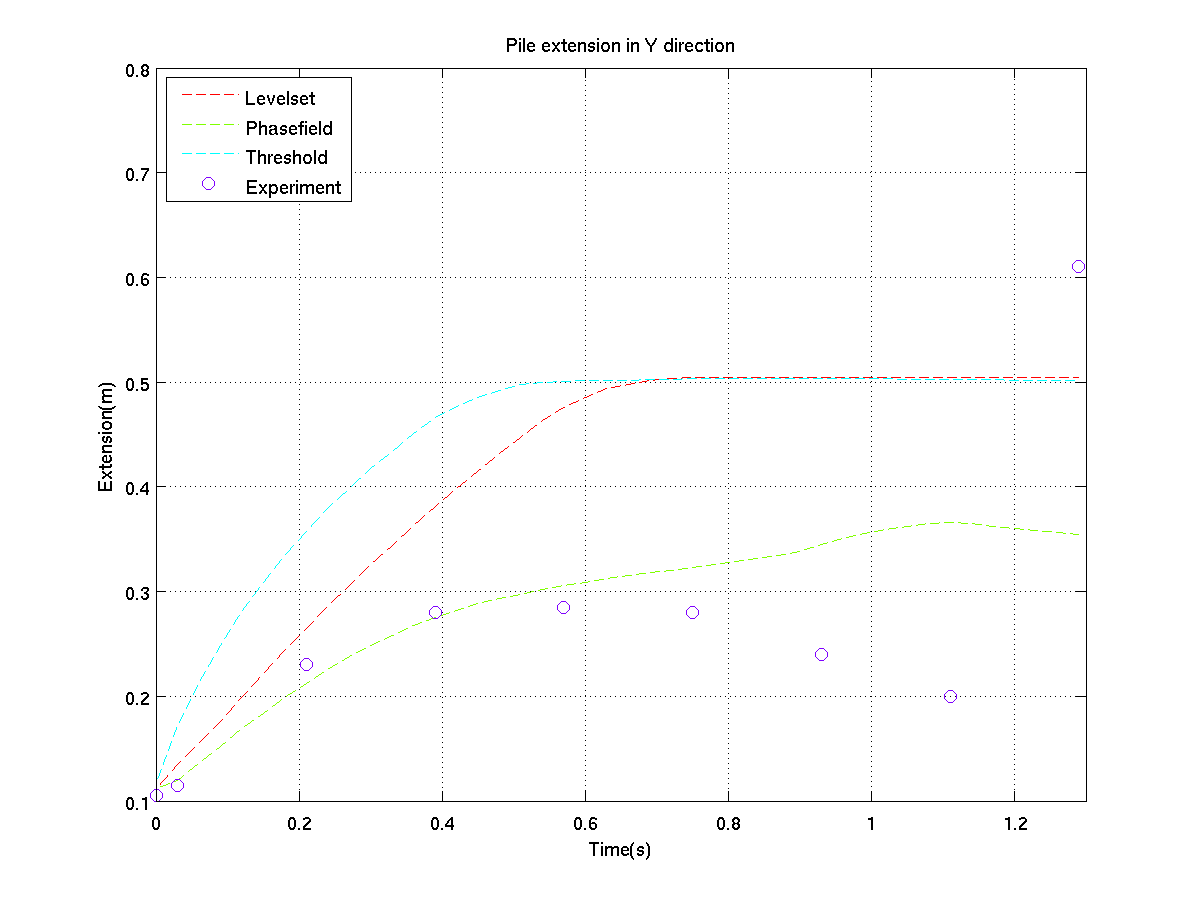
\includegraphics[width=1\textwidth]{IMAGES/yextend.png}
                \subcaption{Extension of pile in Y direction.}
                  \label{y_extent}
                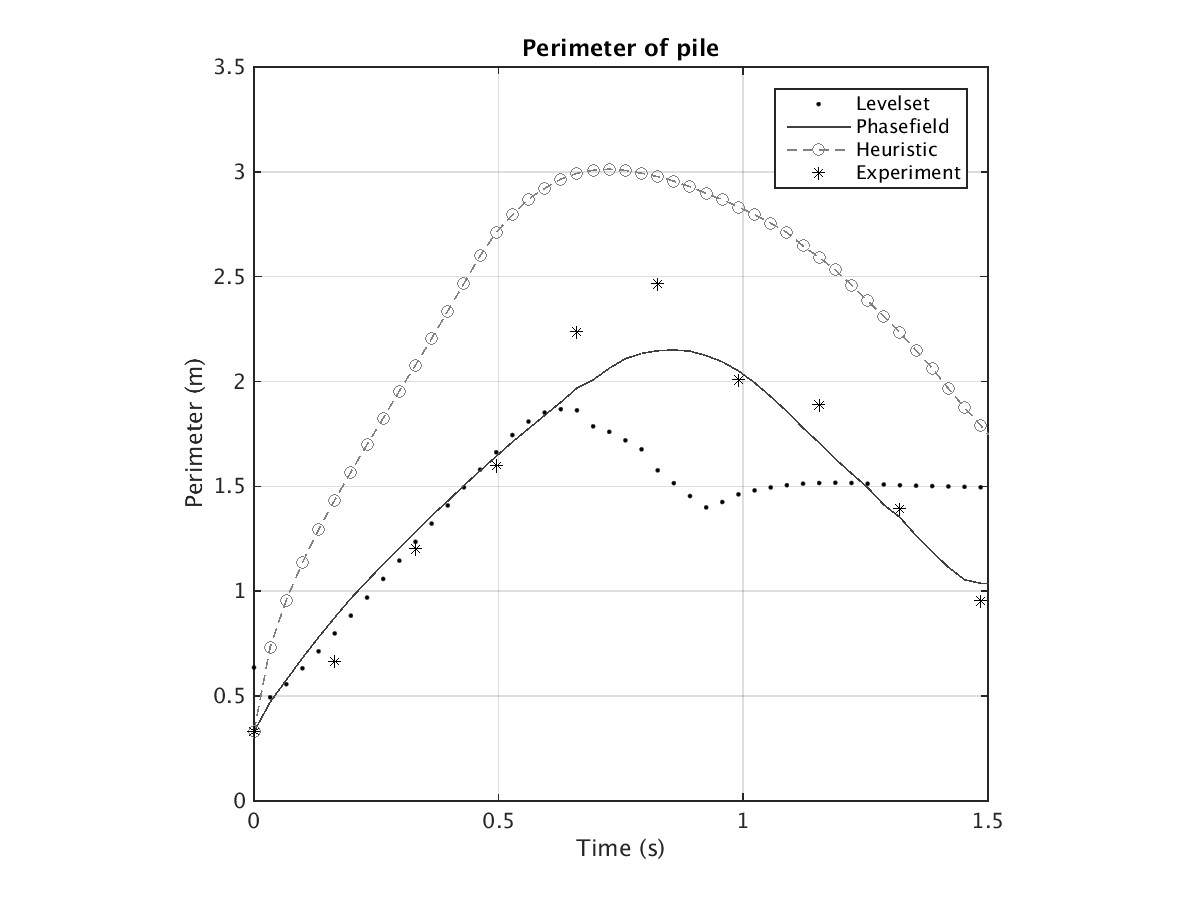
\includegraphics[width=1\textwidth]{IMAGES/perimeter.png}
                \subcaption{Perimeter of pile.}
                  \label{Perimeter}
        \end{minipage}
        \caption{Comparison of the methods for flow on inclined plane.}
        \label{compinc_inclined}
\end{figure}



  
\begin{figure}[H]
        \begin{minipage}[b]{.5\textwidth}
                \centering
                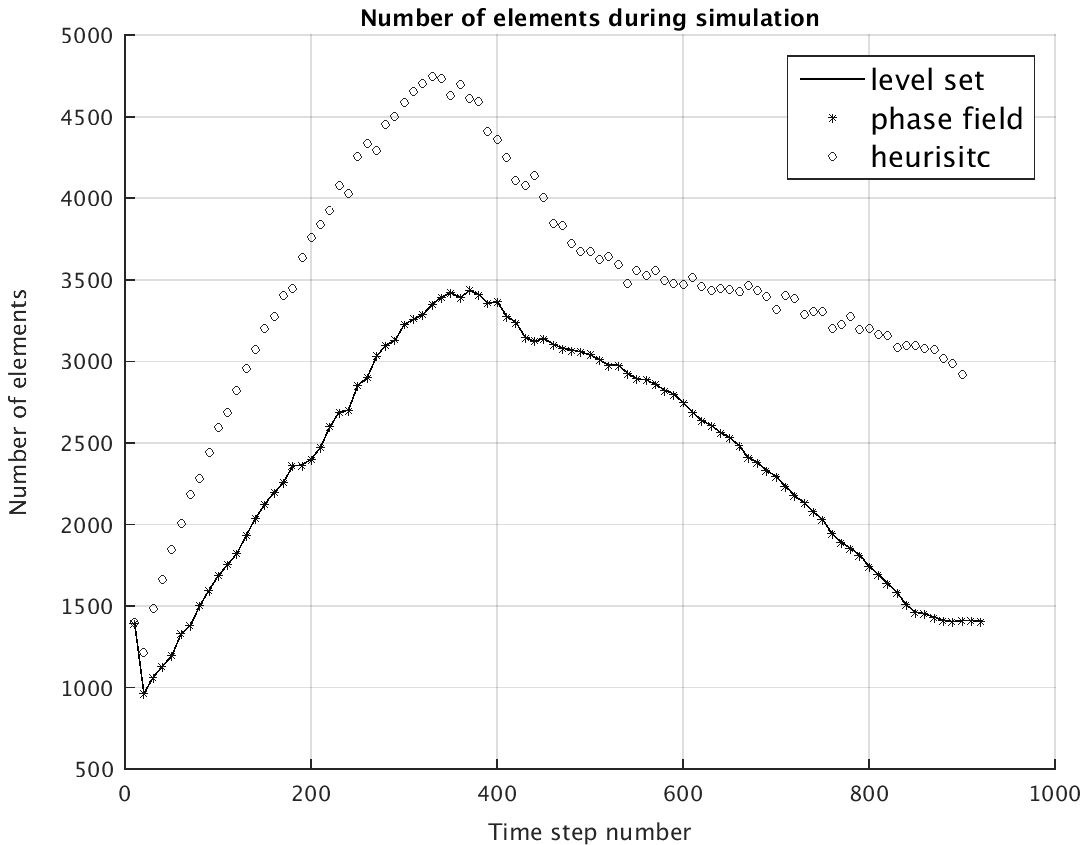
\includegraphics[width=1\textwidth]{IMAGES/incline_num_elem.png}
                \subcaption{Number of the elements for different method of interface capturing during the simulation.}
                \label{mesh_inc}
                
        \end{minipage}
        %   \hfill
        \begin{minipage}[b]{.5\textwidth}
                \centering
                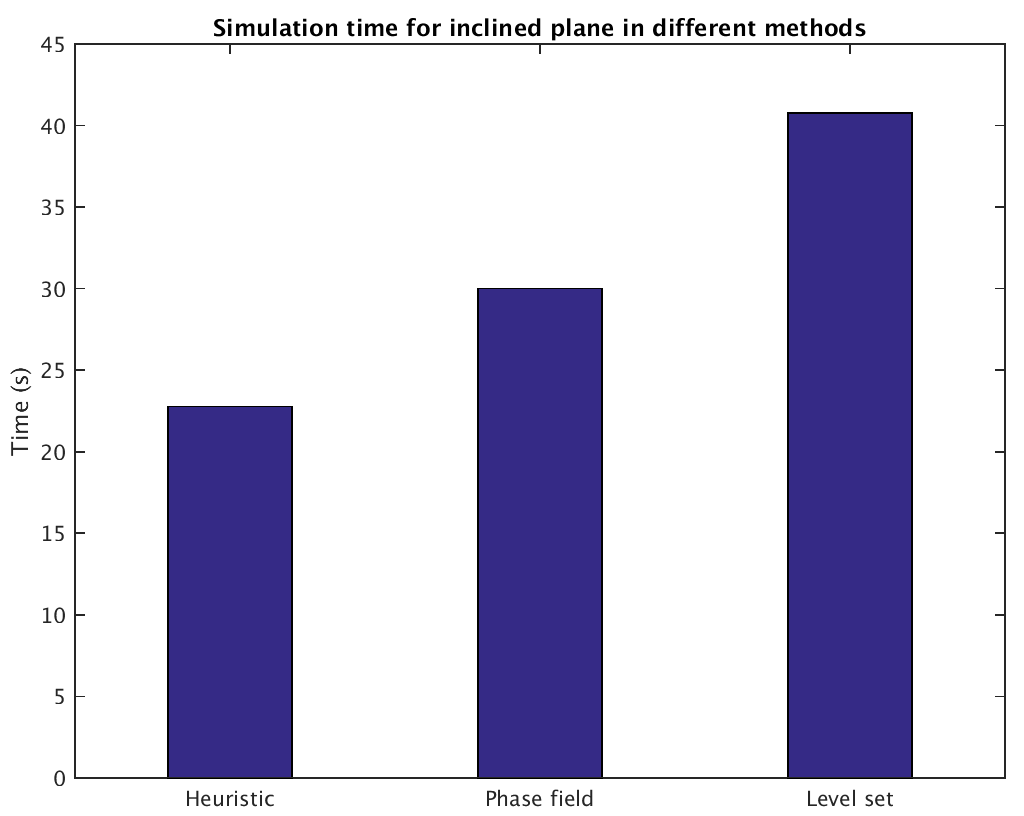
\includegraphics[width=1\textwidth]{IMAGES/incline_timing1.png}
                \subcaption{Time spent for each simulation.\vspace{.375in}}
                \label{barplot_inc}
                
        \end{minipage}
        \caption{Comparison of the methods based on computational cost.}
        \label{compinc_comput}
\end{figure}

Finally, consider the computational cost of the three methods, as shown in figure \ref{compinc_comput}.
The first plot is the number of elements during the simulation and the second one is the wall clock time spent for each simulation.
Since we are using the results of the interface capturing methods for adaptive mesh refinement as described in section \ref{adaptivemeshing}, 
the number of elements during the simulation changes and depends on the different interface capturing methods we use. 
Based on these results, as can be predicted from similarity of the results in the Eulerian interface capturing methods figures \ref{compinc_inclined} 
and \ref{Pile_height_contour}, both Eulerian interface capturing methods have a very similar number of elements during the simulation while the 
interface capturing with the heuristic method results in a larger number of elements. 
Despite the higher number of elements in the heuristic method, the total time needed to complete a simulation, figure \ref{barplot_inc},
is lowest for the heuristic method. Overall the heuristic method took 70\% of the time required for the Phase Field method and only 55\% 
of the time required for the Level Set method.
All of the simulations were performed on one Intel(R) Xeon(R) CPU E3-1220 v3 3.10GHz. Clearly, there is a tradeoff in accuracy and cost.

% \end{figure}
\subsection{Colima Volcano}
%{\huge keith wants the result of Atentique }\\
In this section, we compare our different interface capturing methods to field data from an eruption of the Colima volcano. 
The Colima volcano in Mexico is one of the most active volcanoes in North America, and this eruption happened on 16-17 April 1991 \cite{Charbonnier2008}. 
\begin{center}
        \begin{tabular}{|l|c|}
%               \hline
%               Colima volcano input parameters
                \hline
                Pile shape       & Parabolic \\
                \hline
                Location of pile in X     & 644956.0 \\
                \hline
                Location of pile in Y     & 2157970.0 \\
                \hline
                Maximum pile height       & 30 m \\
                \hline
                Major extent of the pile  & 55 m \\
                \hline
                Minor extent of the pile  & 55 m \\
                \hline           
                Bed friction angle        & $37^o$ \\
                \hline
                Internal friction angle  & $20^o$ \\
                \hline
                Physical time simulated  & 3600 sec \\
                \hline
        \end{tabular}
\end{center}
The topography of the Colima volcano is such that small changes in the initial location of the pile leads to a completely different 
path of flow, so good performance of any of the interface capturing methods for this case promises a reliable method for other volcanoes. 
Unfortunately, only in very rare cases is data during a volcanic eruption available, and thus we cannot perform a direct comparison between the numerical results 
with time-resolved field data.
Usually, for such applications, the deposit of the volcanic event is used to find the outline of the flow and to validate the numerical results.

In figure \ref{Colimapic} we compared the results of the three methods with the outline of the flow from the eruption obtained from the field data \cite{Rupp2006}. 
In the numerical simulations, the outline of the flow is the boundary between wet and dry areas of the domain for whole the simulation. In other words, the points where the flow has
passed are inside the outline, while the rest of the points are located outside of the outline of the flow. 

As in the inclined plane case, we use the same definition for the interface.
Thus $\phi=0$ and $\varPsi=0$ are used for the Phase Field and the Level Set methods, respectively, and $h=\sqrt[3]{Vol} \times {\rm\verb1GEOFLOW_TINY1} $ 
is used for the heuristic method to determine the wet and dry areas.
 
The resolution of the digital elevation model (DEM) of Colima volcano that we use here is 5 meters, which is the finest DEM 
that we have ever used for this volcano.
The outline of this eruption is available in \cite{NamikawaPhD}.
We used the Keyhole Markup Language (KML) to plot the results on real terrain information by using the Google earth application \ref{Colimapic}. 

In figure \ref{colima_outline} one can see the plotted outline of the eruption on Colima volcano. 
This outline is compared to the numerically determined results in figure \ref{Colimapic}.

\begin{figure}[H]
\centering
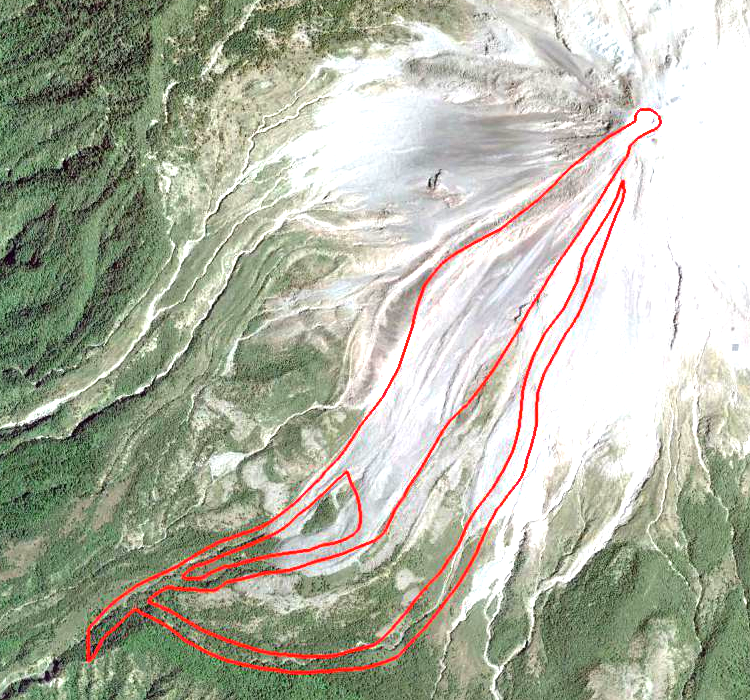
\includegraphics[width=.5\textwidth]{IMAGES/outline1.png}
\caption{Outline of flow for Colima volcano for eruption 16-17 April 1991.}
 \label{colima_outline}

\end{figure}

\begin{figure}[H]
\begin{minipage}[b]{.5\textwidth}
        \centering
                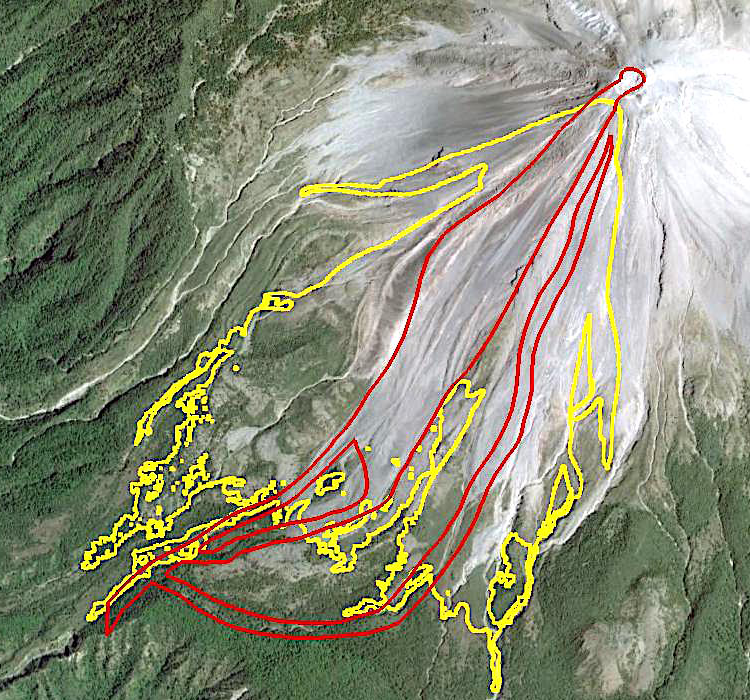
\includegraphics[width=1\textwidth]{IMAGES/tiny1.png}
                \subcaption{Outline from Heuristic Method.}
                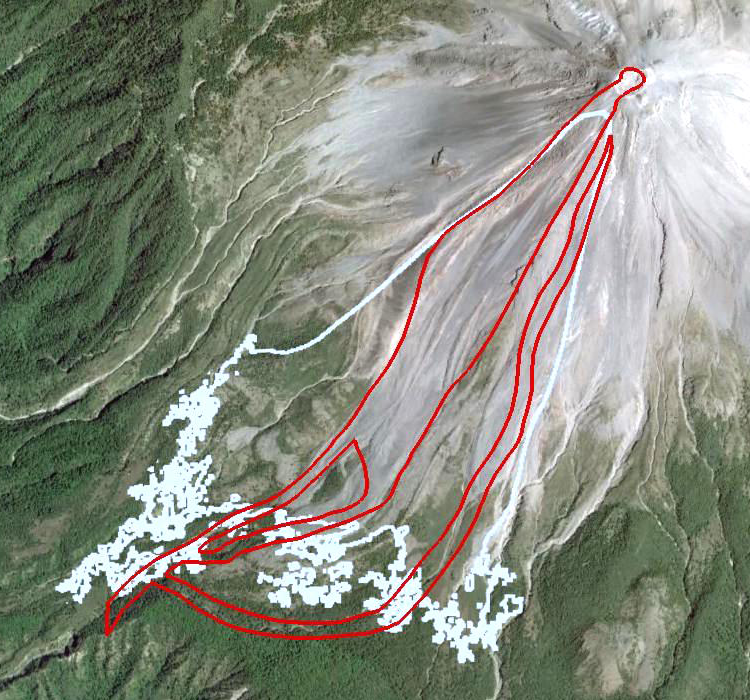
\includegraphics[width=1\textwidth]{IMAGES/levelset1.png}
                \subcaption{Outline from Level Set Method.}
\end{minipage}
        %   \hfill
\begin{minipage}[b]{.5 \textwidth}
                \centering
                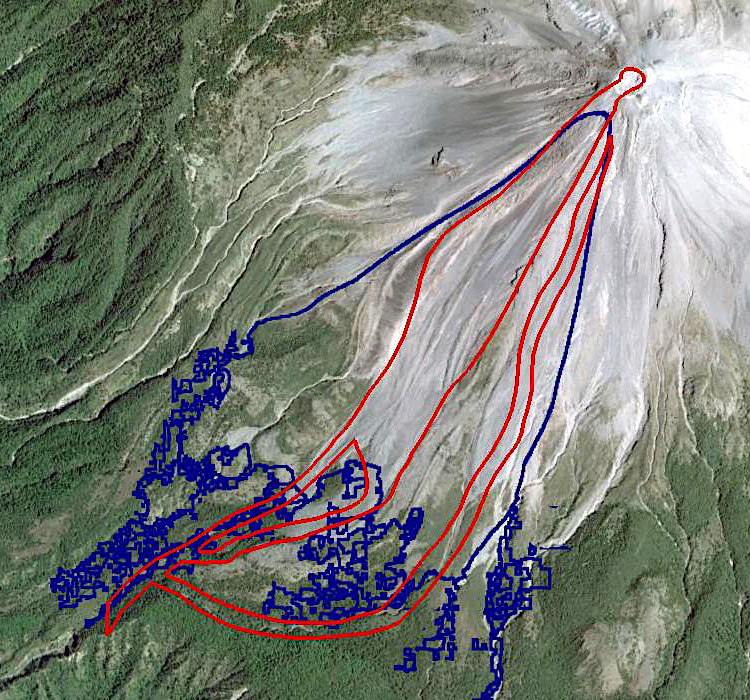
\includegraphics[width=1\textwidth]{IMAGES/phasefield1.png}
                \subcaption{Outline from Phase field Method.}
                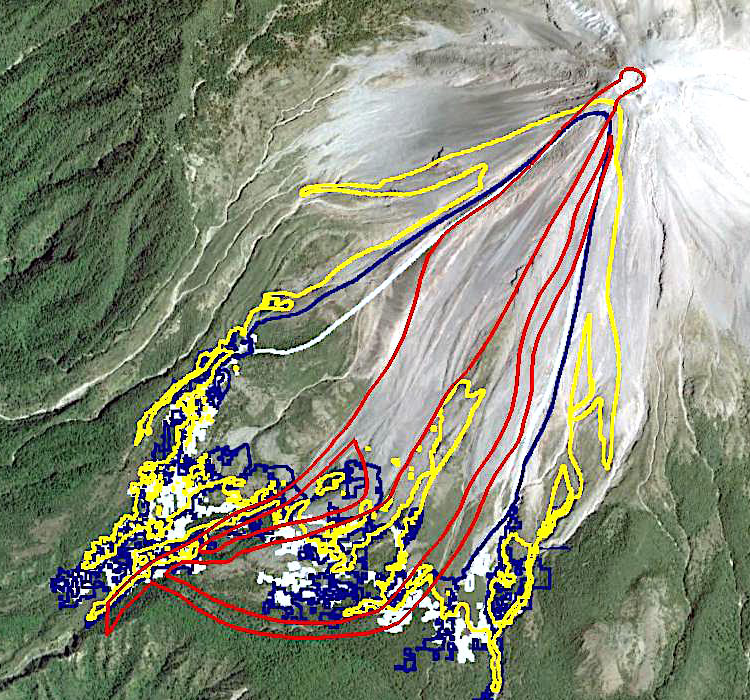
\includegraphics[width=1\textwidth]{IMAGES/comparison1.png}
                \subcaption{Comparison of all three methods.}
        \end{minipage}
        \caption{Comparison of the obtained outline of flow from Heuristic, Level Set, and Phase field methods for Colima Volcano.}
        \label{Colimapic}
\end{figure}

Results of figure \ref{Colimapic} show that all of the methods are successful in controlling the thin layer problem. 
The length of the flow has been captured in all of the methods very well.  This is very important for generating hazard maps. 
The width of the flow is also reasonable in all of the three methods, although the Eulerian methods are slightly more accurate.
The heuristic method captures the separation of the flow into two channels that can be seen in the field deposit data. The heuristic method 
also indicates the presence of two small channels that are not present in the field outline. Note that we are comparing deposits to 
field data.
\begin{figure}[H]
        \begin{minipage}[b]{.5\linewidth}
                \centering
                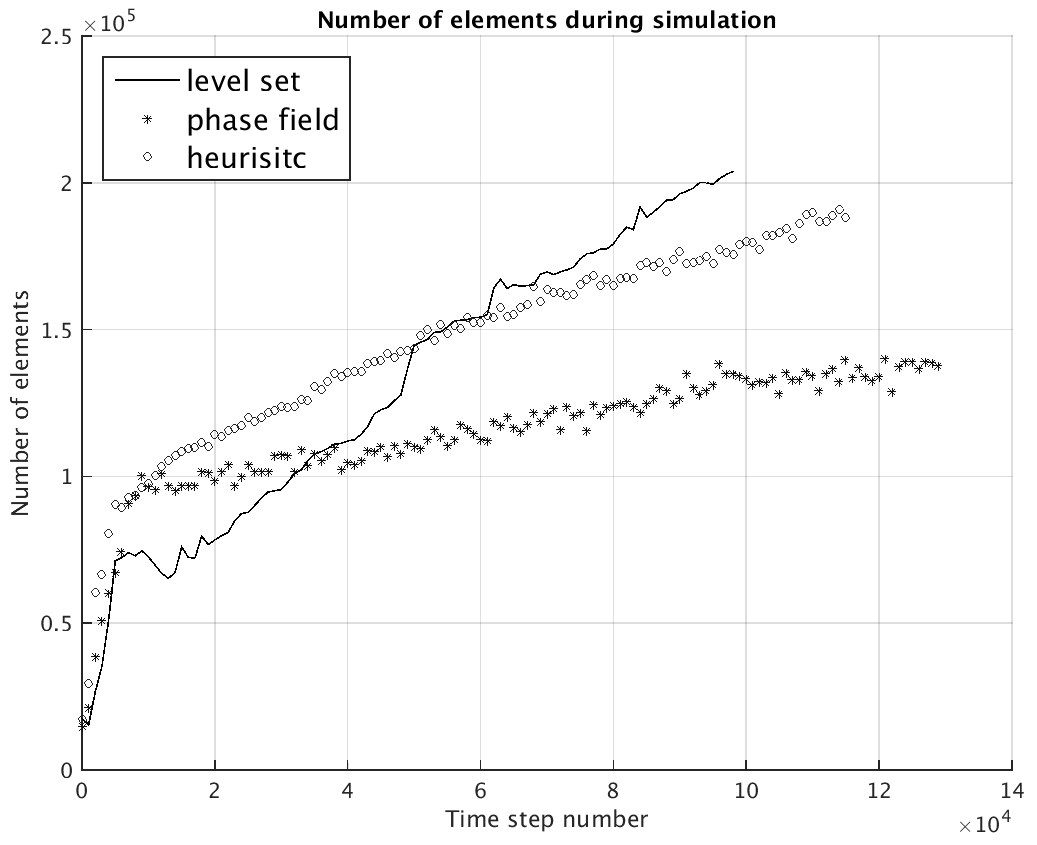
\includegraphics[width=1\textwidth]{IMAGES/colima_num_elem.png}
                \subcaption{Number of the elements for different method of interface capturing during the simulation.}
                \label{col_amr}
                
        \end{minipage}
        %   \hfill
        \begin{minipage}[b]{.5 \linewidth}
                \centering
                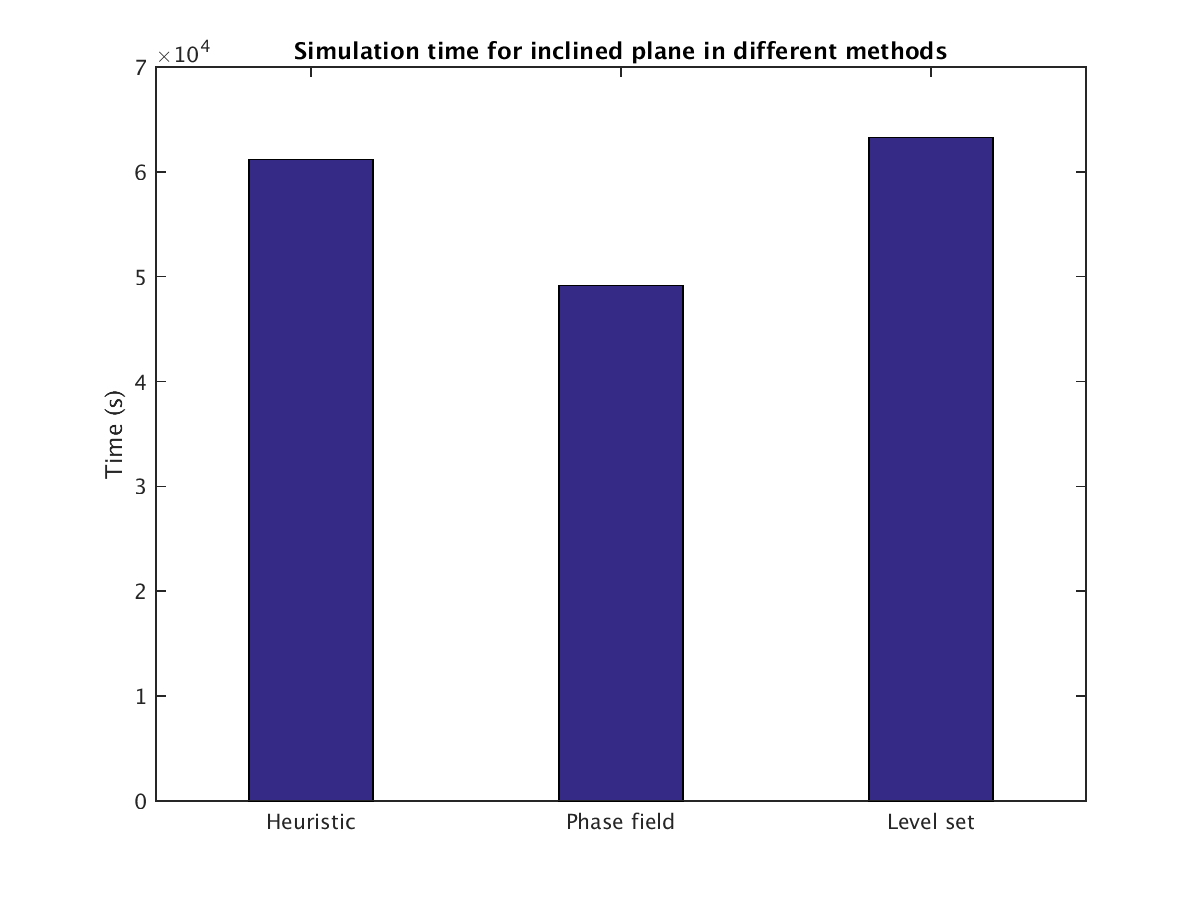
\includegraphics[width=1\textwidth]{IMAGES/colima_timing1.png}
                \subcaption{Time spent for each simulation.\vspace{.4in}}
                \label{comp_col}
        \end{minipage}
        \caption{Comparison of the methods based on computational cost.}
        \label{compinc}
\end{figure}

The computational cost comparison of the methods for the Colima volcano simulations is shown in figure \ref{compinc}. 
We used 16 x 2.27GHz Intel(R) Xeon(R) L5520 for this case. Figure \ref{col_amr} shows the number of the elements during the simulation for the three methods.  
This figures shows the heuristic method and level set have a higher number of elements than the phase field method, 
and both require a higher number of iterations to perform 1 hr physical time simulation. 
The right figure (figure \ref{comp_col}) shows the required time for the simulation. 
In this figure, we can see all of the methods take almost the same amount of computational time, which means that although the 
Level Set and the Phase Field methods are more computationally expensive per time step, the lower number of elements and lower
number of iterations help them to have the same computational cost as the heuristic method.  

\section{Conclusions} \label{conclusions}
The numerical solution of the Savage-Hutter (and similar 
``shallow-water'') equations have historically been plagued by 
several interrelated numerical difficulties which are collectively characterized by a non-physically thin-layer extending large distances from the realistic main body of the flow. 
In the best case, this ``thin-layer problem'' means a ``no flow'' boundary line must be arbitrarily drawn at some given depth contour.  In 
the worst case, it can cause severe numerical instability that 
prevents any simulation of a particular event.
In this paper, we 
have described some features of the thin-layer problem,
some underlying causes that are common to virtually all numerical 
solution methodologies for SW equations. We presented a heuristic method and compared it to two Eulerian interface capturing approaches, namely phase field and level set
based methods, that 
mitigate this problem. In the heuristic method we used a threshold to distinguish between the wet and dry areas, and in the level set and phase field methods, we solved a 
transport equation that implicitly represents the interface of the flow. Then we used the result of a previous step for mesh refinement in all of the three solvers to control 
the thin layer problem and other related problems. Moreover, in the heuristic approach, we also used this result for interface reconstruction and the adjustment of the flux. 
We implemented these thin-layer control strategies in TITAN2D, our high 
performance finite volume solver of the depth-averaged granular 
flow equations. Numerical simulations were performed for two different geophysical mass flows.
To test the solvers, numerical experiments were conducted for an inclined plate and the Colima volcano. For the first case we compared the numerical results 
with experimental results, and for the second case we compared the results with field data. These analyses show that with all of the approaches,
we not only prevented the loss of numerical stability but also demonstrated behavior that is consistent with observations of the flows. In the case of the inclined plane
the phase field and level sets also appear to capture flow outlines more accurately.
%
%As the second case, we tested our solvers on Colima volcano, which is an active volcano 
%in Mexico, was selected on the basis that the DEM had provoked 
%thin-layer numerical difficulties from an earlier version of TITAN2D, 
%and that a campanologist familiar with the location had selectively 
%tuned TITAN2D's few input parameters and also computational and 
%post-processing thresholds to produce results that closely matched 
%reality for that location. The new version of TITAN2D, which implemented
%our thin-layer control strategy, automatically (i.e. without 
%tuning) reproduced a flow outline that had even greater agreement 
%with the historical data. 
%
%Then the results of these approaches were compared. The result of this comparison showed 
%a very good consistency between these approaches.
% Therefore the phase field method could be used for finding the flow boundary 
% of flow and handle the WD problem. 
On the basis of these very positive results, we conclude that our 
thin-layer control strategy, and interface capturing approach provides sufficient benefit. 
While all of these approaches to thin-layer mitigation were developed in the 
context of TITAN2D and granular flows, much of it should be appropriate 
for use in depth-averaged flow solvers with different numerical 
schemes and physics.

%\appendix
\section*{Acknowledgements}
 We acknowledge the Colima deposit  and experiment data made available to us by Prof. M. I. Bursik and for helpful discussions on the use of that data.

\section*{References}

\bibliography{mybib}

\end{document}
